Enter some blurb here for a short introduction to content

\subsubsection{Model parameters and simulation setup}\label{sec:parameters}

The dynamics of the binary fluid mixture is governed by inertial,
viscous, and surface tension forces. The relative magnitudes of these
forces at a characteristic length scale \(L\) and characteristic
velocity \(U\) are captured by the capillary number $\mathrm{Ca}=\frac{\eta U}{\sigma}$ and the Weber number
\(\mathrm{We}=\frac{\rho U^2 L}{\sigma}\). Here we are primarily interested in spinodal decomposition of the mixture, 
where we analyze the dynamics after the initial formation of the interfaces and neglect residual diffusion. Hence the 
Peclet number \(\mathrm{Pe}=\frac{UL}{\Gamma}\) is of lesser importance and we do not consider it when choosing our 
simulation parameters.

The equations of motion of our model comprise the relevant materials
properties: the density \(\rho\), viscosity \(\nu\), and surface tension \(\sigma\) of the binary fluid, and the mass \(m_p\), size \(R_p\) and aspect ratio \(\alpha\), and dipole moment \(m\) of the particles. In addition, we can control the particle volume fraction \(\phi_p\) and
magnetic field strength \(B\). These nine quantities involve four unit
dimensions (mass, length, time, and charge), hence we can use five
dimensionless variables to specify the parameters of the system. These
are the particle aspect ratio $\alpha$, particle volume fraction
\(\phi_p\), particle vs.~fluid density ratio
$\xi = \frac{3m_p}{4\pi \rho V_p}$, nominal Weber number $\mathrm{We} = \frac{\rho \sigma V_p^{1/3}}{\eta^2}$, and magnetic Bond
number \(\bar{B} = m B/(\sigma A_p)\), where
\(V_p=(4/3)\pi R_\parallel^3/\alpha^2\) is the particle volume and
\(A_p=\max\left( \pi R_\parallel^2/\alpha, \pi R_\parallel^2/\alpha^2 \right)\)
the area of the larger cross-section of the ellpsoidal particles.

For our simulations, we choose units \(\Delta x\), \(\Delta t\),
\(\Delta m\), and \(\Delta i\) such that \(V_p=\hat{V}_p(\Delta x)^3\),
\(\nu=\hat{\nu}(\Delta x)^2/\Delta t\),
\(\sigma=\hat{\sigma}\Delta m/(\Delta t)^2\), and
\(m=\hat{m}\Delta i(\Delta x)^2\). We used \(V_p=2000\pi/3\),
\(\hat{\nu}=1/6\), \(\hat{\sigma}=0.0267\), \(\hat{m}=1\), and a density
ratio \(\xi=1/\hat{\rho}\). For reference, the values of the model
parameters are listed in table \ref{tab:parameters}. The values of
\(\alpha\) and \(\bar{B}\) are variable and are reported
with the results in section \ref{sec:results}.

%\new{We note that the dynamics of the simulations are determined by
%the dimensionless numbers, and the actual unit values $\Delta x$,
%$\Delta t$, $\Delta m$, and $\Delta j$ are arbitrary and only become
%meaningful when a connection to an experimental system is made (see
%below).}

\begin{table}
\centering
\caption{Summary of the parameters of the numerical model and the values used in the simulations}
\label{tab:parameters}
\begin{tabular}{|c|r|}
\hline
Parameter & Value \\
\hline
$L_V/\Delta x$ & 256 \\
$\rho \cdot (\Delta x)^3/\Delta m$ & 0.7 \\
$\nu \cdot \Delta t/(\Delta x)^2$ & 1/6 \\
$\sigma \cdot (\Delta t)^2/\Delta m$ & 0.0267 \\
$\tau/\Delta t$ & 1 \\
$g \cdot \Delta m(\Delta t)^2/(\Delta x)^5$ & 0.08 \\
$\phi_f$ & 0.5 \\
$\phi_p$ & 0.15 \\
$n_p$ & 1200 \\
$\rho_p \cdot (\Delta x)^3/\Delta m$ & 1 \\
$V_p/(\Delta x)^3$ & $2000\pi/3$ \\
$m/(\Delta i(\Delta x)^2)$ & 1 \\
$d_c/\Delta x$ & 2/3 \\
$K_H\cdot (\Delta x)^{1/2}(\Delta t)^2/\Delta m$ & 100 \\
\hline
\end{tabular}
\end{table}

We performed simulations of a binary fluid using the software package
LB3D \cite{schmieschek_lb3d_2017} that implements the lattice Boltzmann method described in section
\ref{sec:methods}. The multicomponent
lattice Boltzmann model is solved in a cubic box of size
\(L_V=256\Delta x\) with periodic boundary conditions. The simulation
box is filled with equal volume fractions \(\phi_f=0.5\) of two fluids,
initially homogeneously mixed with a density
\(\rho=0.7\Delta m/(\Delta x)^3\). The BGK relaxation time is set to
\(\tau=\Delta t\) and the Shan-Chen interaction strength is set to
\(g_{kk^\star}=0.08(\Delta x)^2/(\Delta m(\Delta t)^2)\). We performed
preliminary simulations of a spherical droplet with these parameters and
fitted the pressure difference inside and outside the droplet to the
Young-Laplace law, which yielded a surface tension
\(\sigma=0.0267\Delta m/(\Delta t)^2\). To study the influence of
anisotropic particle shapes on the bijel formation, we performed
simulations for particles with three different aspect ratios:
\(\alpha=1\) for spherical particles, \(\alpha=2\) for prolate
ellipsoids, and \(\alpha=1/2\) for oblate ellipsoids. To match the
particle volume fraction \(\phi_p\) between the different particle
shapes, we kept the volume of the particles fixed and used the same
number of particles for each aspect ratio. The radius along the symmetry
axis of the particles was calculated from
\(V_p=(4/3)\pi R_\parallel^3/\alpha^2\), yielding
\(R_\parallel=7.9\Delta x\) for spheres, \(R_\parallel=12.6\Delta x\)
for prolate ellipsoids, and \(R_\parallel=5\Delta x\) for oblate
ellipsoids, respectively. Particles were added to the fluid by placing
them randomly inside the box. The lubrication cutoff distance was set to
the value \(d_c=(2/3)\Delta x\) recommended by Ladd
\cite{ladd_lattice-boltzmann_2001}, and the strength of the Hertz
potential was set to \(K_H=100\Delta m/((\Delta x)^{1/2}(\Delta t)^2)\).
We first equilibrated the particle positions and orientations by
evolving only the equations of motion of the particles, while the fluid
remained in its initial configuration, until the minimum particle
distance exceeded \(1.2\cdot\max(R_\parallel,R_\parallel/\alpha)\).
After the equilibration, the magnetic flux density
\(\vec{B}=B\hat{\vec{z}}\) was switched on and the full system was
evolved for \(10^5\) timesteps. In the course of the simulation, the binary mixture undergoes spinodal decomposition. 
The particles adsorb at the coarsening interface and eventually become jammed, resulting in the bicontinuous phase 
morphology of the bijel.

It is worth discussing briefly the possible realization of our model in
experiments. A common choice for bijel formation in binary liquids is a
mixture of water and lutidine
\cite{clegg_emulsification_2007,herzig_bicontinuous_2007}. The surface
tension between the phases of a water-lutidine system at
\(40^\circ\mathrm{C}\) is around \(\sigma=0.22\ \mathrm{mN/m}\) and the
dynamic viscosity of the lutidine-rich phase is around
\(\eta=2.38\ \mathrm{mPa\,s}\) \cite{grattoni_lower_1993}. Ellipsoidal
particles with various aspect ratios can be formed by mechanically
stretching spherical particles \cite{trevenen_gradient_2021}. Such
particles can be magnetically functionalized by e-beam deposition of a
Nickel layer. Fei et
al.~\cite{fei_magneto-capillary_2018,fei_magneto-capillary_2020}
fabricated coated \(4\ \mathrm{\mu m}\) polystyrene particles with a
permanent magnetic dipole moment of
\(m\approx3\cdot10^{-14}\ \mathrm{Am^2}\). It was shown that the dipole moment is oriented in the direction parallel to the coated interface \cite{yan_linking_2012,yan_rotating_2014}, i.e., it can be aligned with the axis of ellipsoidal particles.
For the given surface tension, the capillary torque on a particle adsorbed at an interface is approximately
$8.8\cdot10^{-16}\ \mathrm{Nm}$. We thus can estimate that a magnetic
flux density of \(30\ \mathrm{mT}\) is able to exert a magnetic torque
that exceeds the capillary torque.
We note that under these conditions,
the dipole-dipole interaction is on the order of
\(10^{-16}\ \mathrm{J}\) and an order of magnitude smaller than the
particle-interface interaction which is of order
\(10^{-15}\ \mathrm{J}\). %Unlike previous works
%\cite{xie_direct_2017,xie_controllable_2021}, we therefore cannot
%neglect the magnetic dipole-dipole interactions between particles.For these bijel properties and the parameters given in
table \ref{tab:parameters}, the spatial resolution of our
simulations is $\Delta x\approx252\ \mathrm{nm}$, and the time step
is $\Delta t=624\ \mathrm{ns}$. This corresponds to a system side length of $L_V \approx 64.5\ \mathrm{\mu m}$ and a runtime of
$T \approx 62.4\ \mathrm{ms}$.

\begin{figure}
\centering
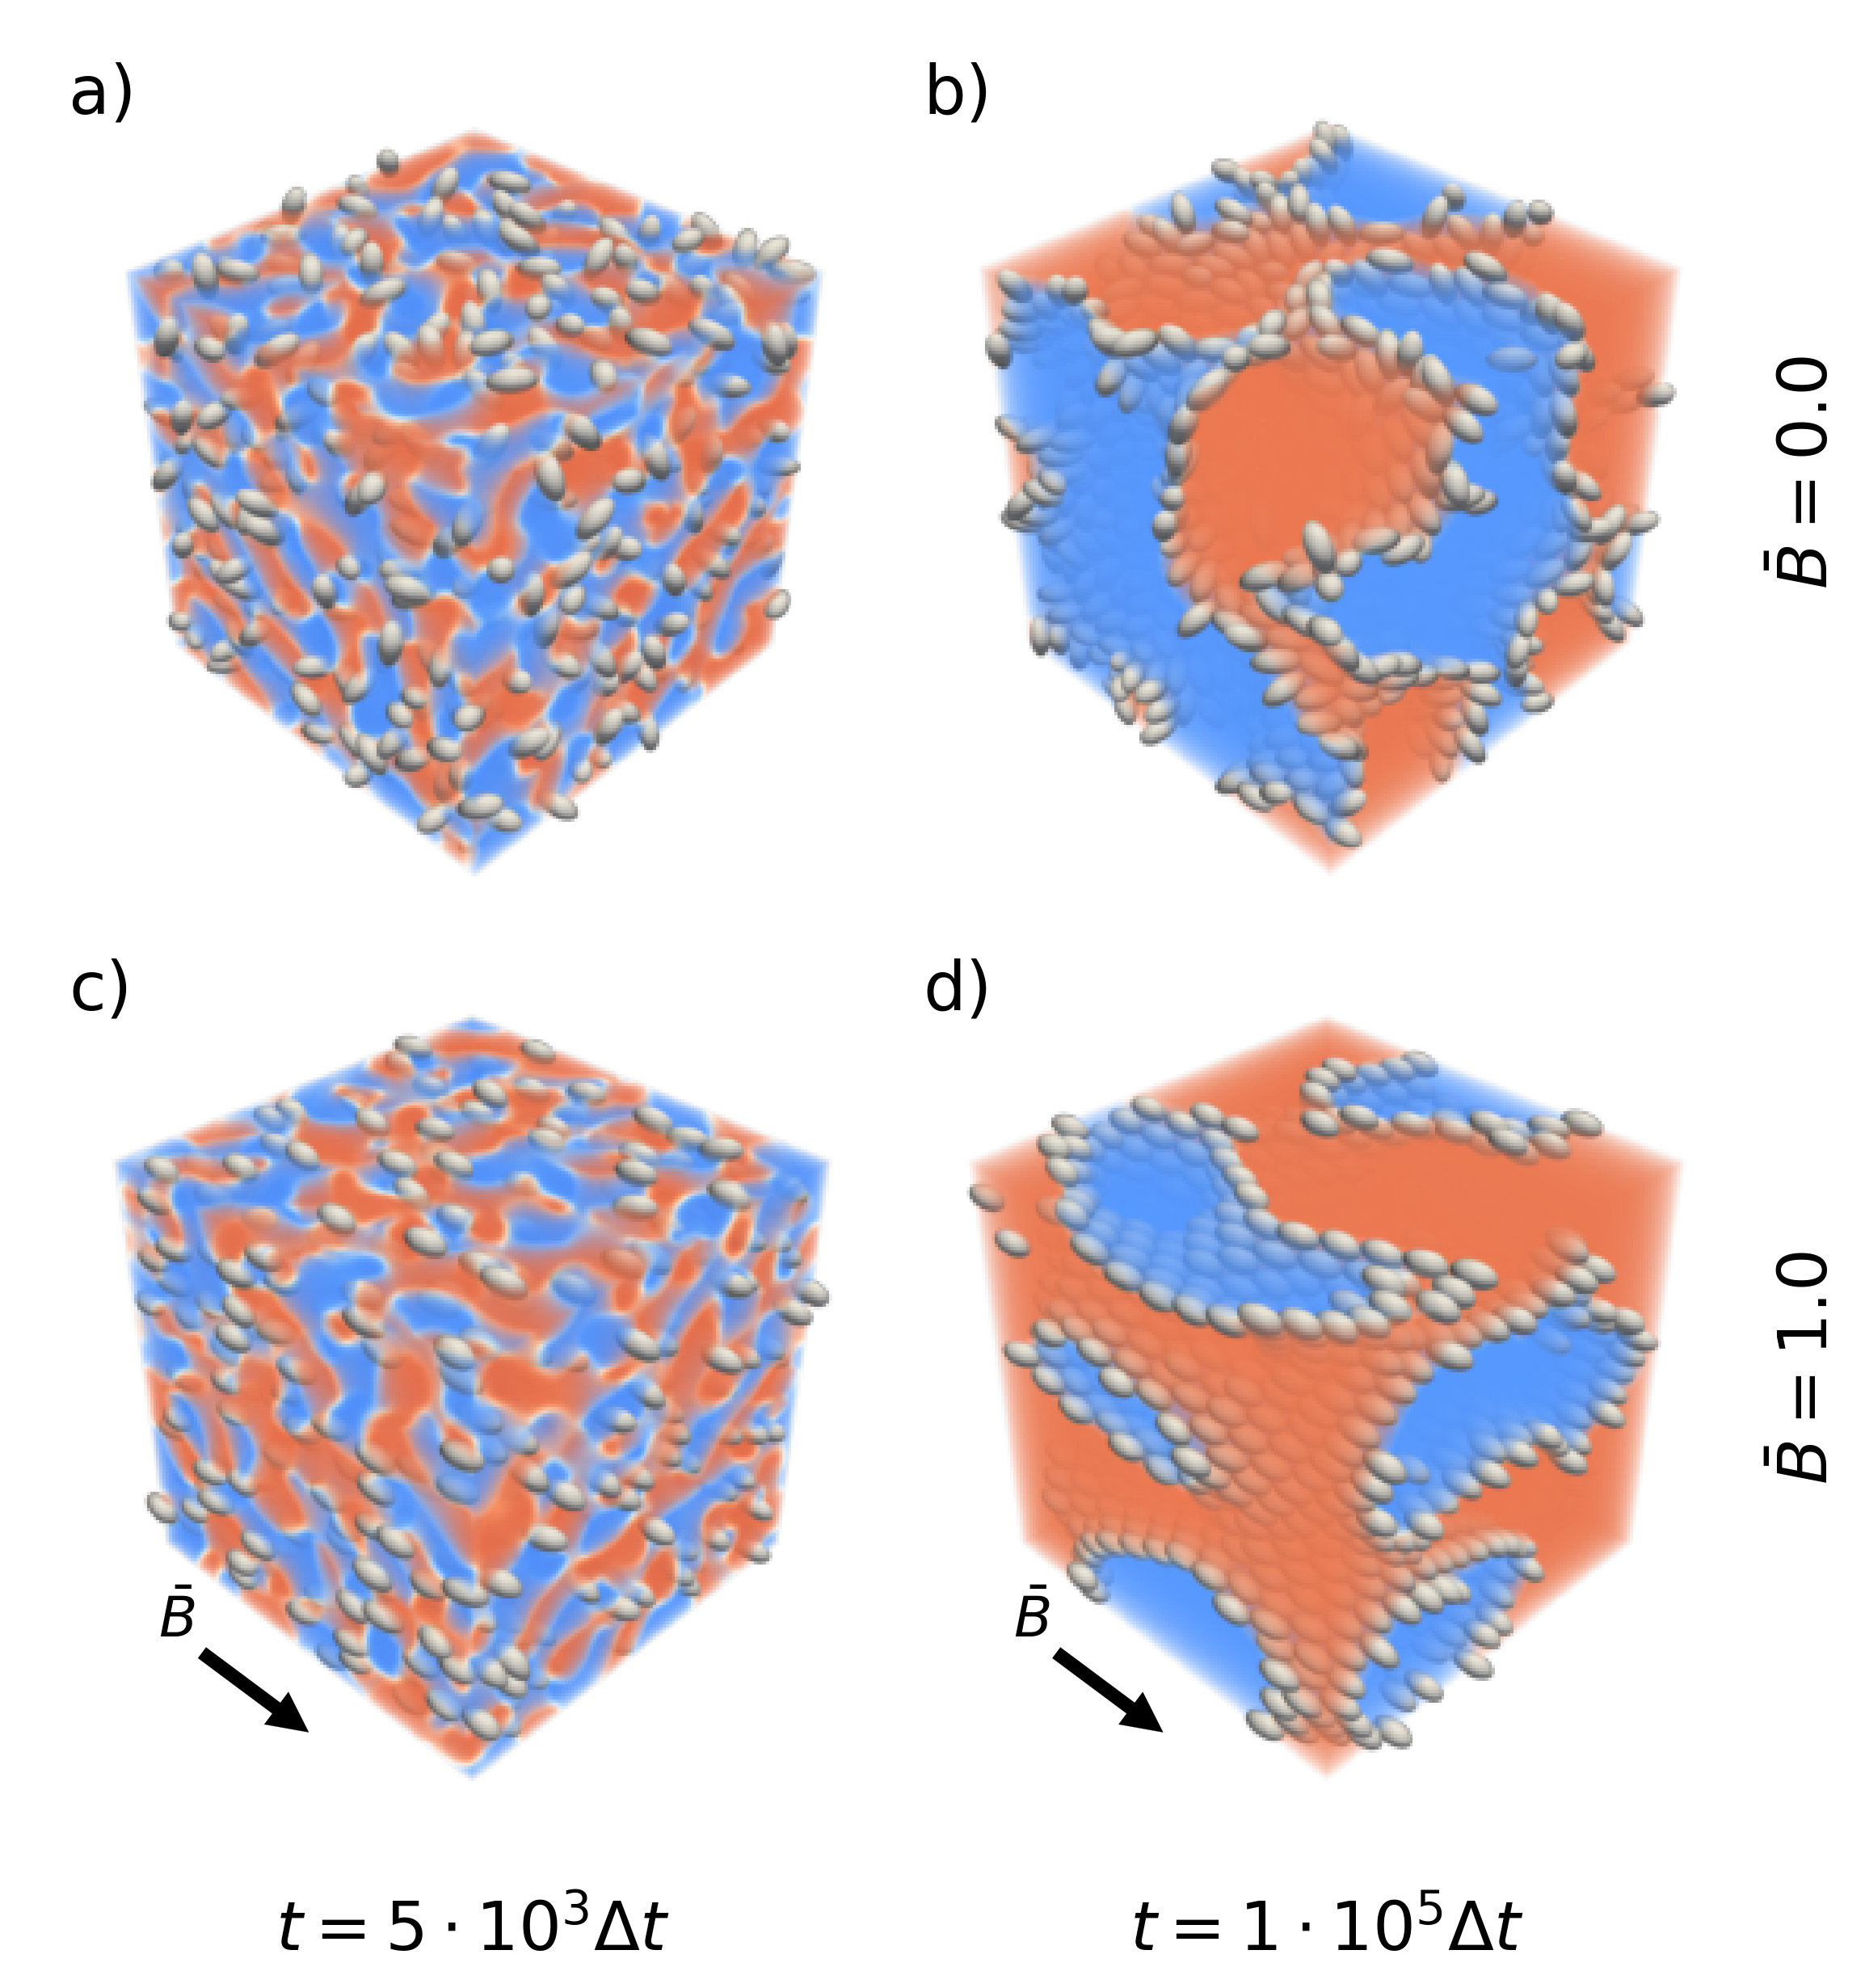
\includegraphics[width=\columnwidth]{figures/results/paper1/microstructure_viz.png}
\caption{Snapshots of emulsion gels stabilized by prolate ellipsoids after $t=5\cdot10^3$ timesteps (left) and after $10^5$ timesteps (right). The top row shows the structure forming without a magnetic field. The bottom row shows the structure forming in an applied magnetic field of reduced strength $\bar{B}=1.0$. The snapshots are colored according to the order parameter $\phi$.}
\label{fig:microstructure_viz}
\end{figure}

\section{Results}\label{sec:results}

\begin{figure*}
\centering
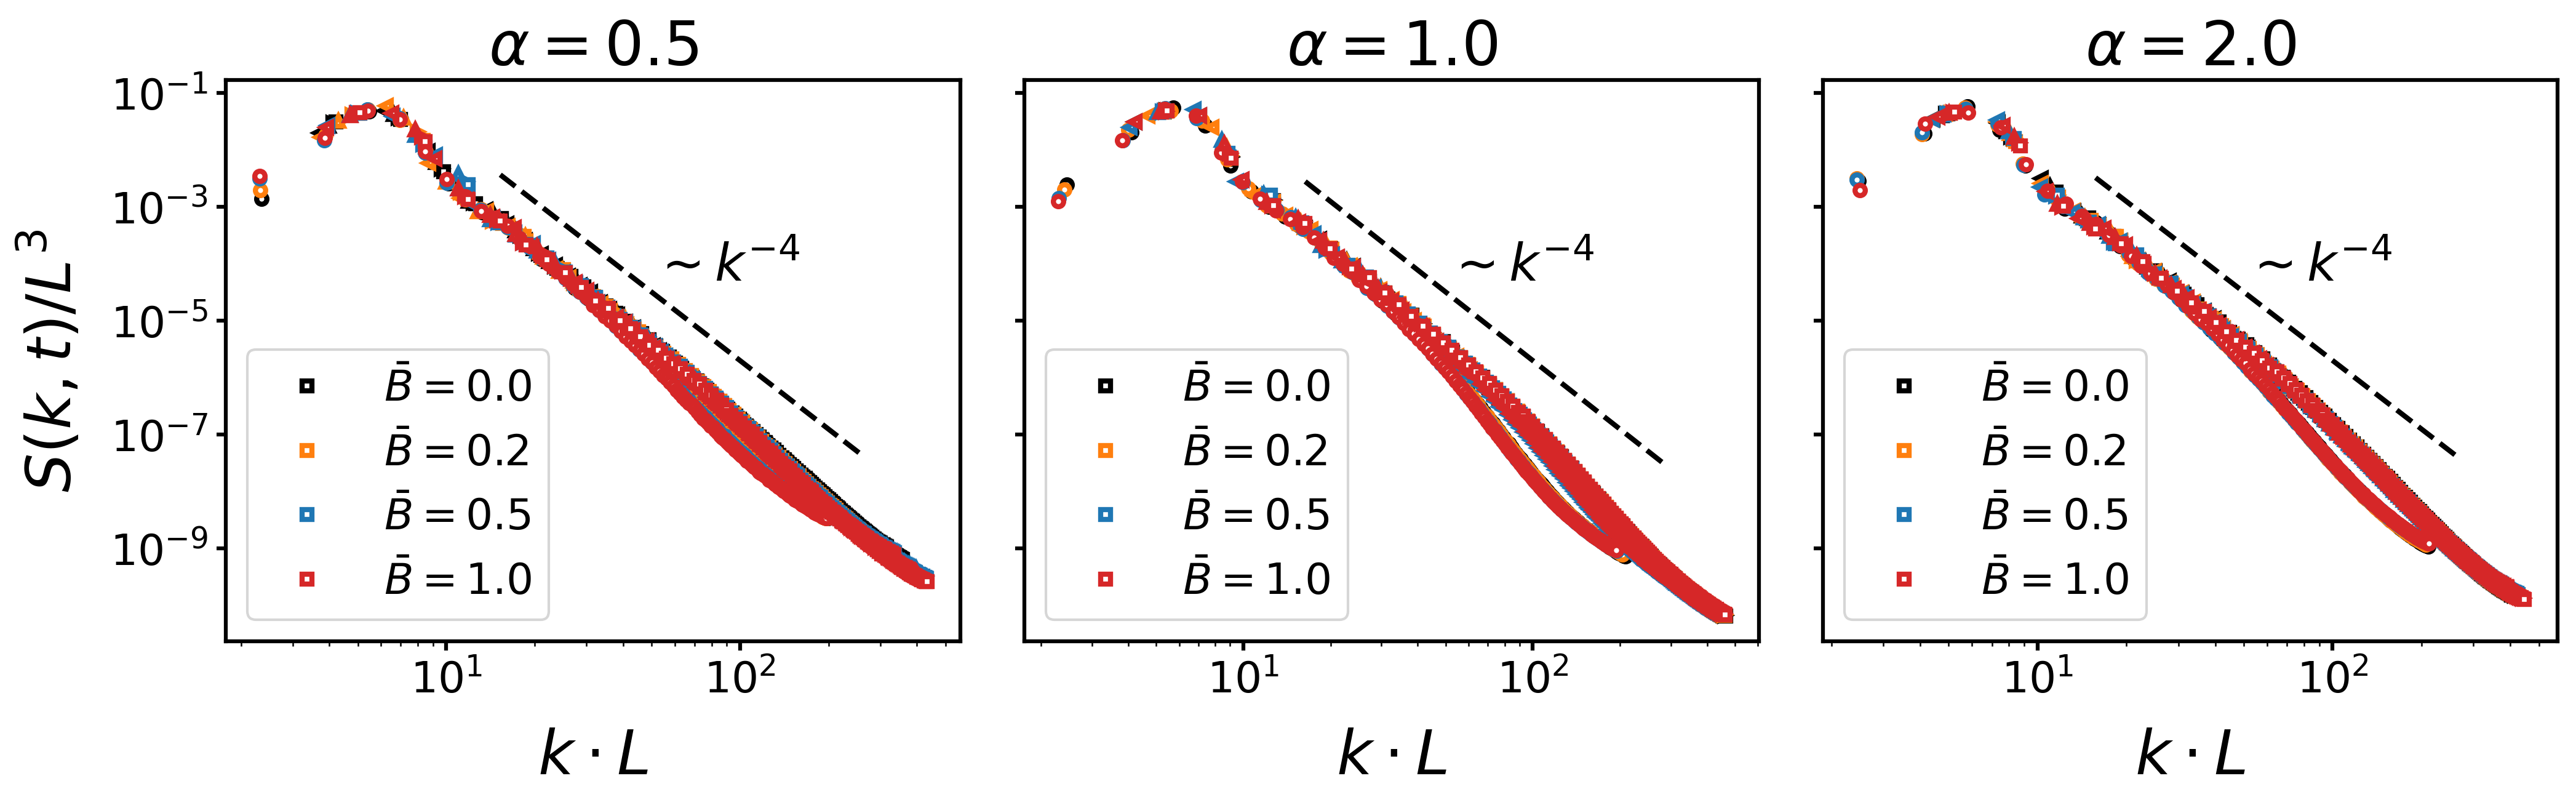
\includegraphics[width=\textwidth]{figures/results/paper1/structure_factor.png}
\caption{Scaling plot of the dynamic structure factor $S(k,t)$ for different particle shapes $\alpha$ and at different magnetic field strength $\bar{B}$. The structure factor is plotted at four different timesteps for each case. The good data collapse shows that the bijel formation is driven by spinodal decomposition. The decay to the right of the peak is reasonably well described by Porod's law $S(k)\sim k^{-4}$.}
\label{fig:structure_factor}
\end{figure*}

Bijels can be used as emulsion templates for porous materials with
applications including drug delivery, water desalination, and battery
electrodes
\cite{vanoli_bijels_2022, chen_pore-scale_2022, lu_controllable_2020, garcia_scalable_2019}.
The transport properties of porous materials depend on the porosity and
tortuosity of the void space and can be linked to the phase-separated
morphology of the bijel template. Therefore, we study the domain size
and tortuosity of the phase morphology of bijels stabilized by
anisotropic particles. In particular, we investigate the effect of
magnetic particles on the microstructure of bijels that are formed in
external magnetic fields. We simulated bijels with a particle volume
fraction of \(\phi_p=0.15\) and varied the magnetic flux density such
that the Bond numbers varies in the range \(0\le\bar{B}\le1\).
In this work, we use a fixed particle volume fraction and focus on the dependence of the bijel structure on the magnetic field. Bijels with varying particle loading and surface tension and have been studied elsewhere in the literature, e.g., by Hijnen et al.\cite{hijnen_bijels_2015} and Jansen and Harting\cite{jansen_bijels_2011}.

Figure \ref{fig:microstructure_viz} shows snapshots of the bijel
microstructure observed at different times with and without an external
magnetic field. The figure illustrates how anisotropic particles align
with the direction of the magnetic field. As the particles reorient,
they can deform the interface which thus responds by rearrangements
including reorientation and domain coalescence or breakup. This results
in apparently larger domain sizes for bijel formation in magnetic
fields. The quantitative effect on the bijel morphology, and domain size
in particular, is analyzed in the following sections.

\subsection{Structure factor and domain size of magnetically responsive bijels}

In LB simulations of spinodal decomposition
\cite{kendon_3d_1999,kendon_inertial_2001}, a characteristic length
scale can be obtained from the structure factor
%
\begin{equation}
S(\vec{k},t) = \tilde{\phi}(\vec{k},t)\tilde{\phi}(-\vec{k},t) .
\end{equation}
%
where \(\tilde{\phi}(\vec{k},t)\) is the Fourier
transform of the order parameter fluctuations
\(\phi(\vec{x},t)-\left\langle\phi\right\rangle\). A common measure of
domain size uses the spherically averaged structure factor
%
\begin{equation}
S(k,t) = \frac{1}{n_k} \sum_{k-\frac{\Delta}{2}<k<k+\frac{\Delta}{2}} \tilde{\phi}(\vec{k},t)\tilde{\phi}(-\vec{k},t) ,
\end{equation}
%
where \(k=|\vec{k}|\) denotes the modulus of \(\vec{k}\)
and \(n_k\) is the number of lattice sites in a shell of radius \(k\)
and thickness \(\Delta=2\pi/L_V\). The average domain size can then be
defined in terms of the \(n\)-th moment of the structure factor
\cite{laradji_molecular_1996}

\begin{equation}
L_n(t) = 2 \pi (\left( \frac{\sum_k S(k, t)}{\sum_k k^n S(k, t)} )\right)^{\frac{1}{n}}
\end{equation}

It is worth noting that this definition of average domain
size does not necessarily yield values that coincide with the typical
domain size observed visually in snapshots such as those shown in
Fig.~\ref{fig:microstructure_viz}. However, in a dynamic
scaling regime, different measures of domain size are expected to differ
only by a constant ratio. We found that the commonly used measure
\(L_1(t)\) tends to overestimate the observed domain size. Numerically,
the calculation of the spherically averaged structure factor is subject
to poor statistics in the low \(k\)-shells, where the average
\(|\vec{k}|\) of the lattice sites differs from the nominal shell
radius. Additionally, the measurement of \(L(t)\) in simulations with
periodic boundary conditions is subject to finite size effects. More
importantly, in suspensions of anisotropic particles, we cannot expect
that the structure factor is isotropic. Therefore, we also used the 3D
structure factor to calculate a lateral domain size in each Cartesian
direction from the second moments
\cite{jansen_bijels_2011,gunther_timescales_2014}
%
\begin{equation}
L_\beta(t)=2\pi\sqrt{\frac{\sum_{\vec{k}}S(\vec{k},t)}{\sum_{\vec{k}}k_\beta^2 S(\vec{k},t)}} .
\end{equation}
%
This allows us to compute a domain size parallel
(\(L_\parallel=L_z\)) and perpendicular (\(L_\perp=(L_x+L_y)/2\)) to the
direction of \(\vec{B}\) separately. The average domain size \(L_d(t)\)
is computed as \(L_d(t)=\sum_\beta L_\beta(t) / 3\).
%
\begin{equation}
L_d(t)=2\pi\sqrt{\frac{\sum_{\vec{k}}S(\vec{k},t)}{\sum_{\vec{k}}\sum_\beta k_\beta^2 S(\vec{k},t)}} .
\end{equation}
%
%In case the structure factor is isotropic
%\(S(\vec{k},t)=S(k,t)\), this is equivalent to the ratio of the fourth
%and second moments of the spherically averaged structure factor.
%
%\begin{equation}
%\begin{split}
%  L_d(t) &%= \left[\sum_{\beta}\left(\frac{1}{L_\beta(t)}\right)^2\right]^{-\frac{1}{2}}
%  = 2\pi \sqrt{\frac{\sum_{\vec{k}}S(\vec{k},t)}{\sum_{\vec{k}}\sum_\beta k_\beta^2 S(\vec{k},t)}} \\
%L_\perp(t) &%= \left[\left(\frac{1}{L_x(t)}\right)^2+\left(\frac{1}{L_y(t)}\right)^2\right]^{-\frac{1}{2}}
%= 2\pi \sqrt{\frac{\sum_{\vec{k}}S(\vec{k},t)}{\sum_{\vec{k}} \left(k_x^2+k_y^2\right) S(\vec{k},t)}} \\
%L_\parallel(t) &= 2\pi \sqrt{\frac{\sum_{\vec{k}} S(\vec{k},t)}{\sum_{\vec{k}} k_z^2 S(\vec{k},t)}}
%\end{split}
%\end{equation}

Before calculating the structure factor \(S(\vec{k},t)\), we
first filled the lattice sites covered by particles with the average
density at the surrounding lattice sites. We employed an iterative
procedure that fills the particles layer by layer, starting at the
surface layer and using equation \eqref{eq:fill_particles} to
approximate the density at solid nodes that have a least one neighboring
fluid node. This is repeated until all solid nodes have been filled with
fluid. The order parameter \(\phi(\vec{x},t)\) was then calculated for
the filled density fields \(\rho_k(\vec{x},t)\). Filling the lattice
sites covered by particles is crucial to avoid spurious oscillations of
the structure factor at length scales corresponding to the particle
size.

Figure \ref{fig:structure_factor} shows the scaling of the dynamic
structure factor \(S(k,t)\). The data collapse is good, albeit
deviations from dynamic scaling are present at smaller length scales.
The decay to the right of the maximum is reasonably well described by
Porod's law \(S(k)\sim k^{-4}\) indicating scattering off a nearly flat
interface. These results are in line with the scaling results by Kendon
et al.~\cite{kendon_3d_1999, kendon_inertial_2001} for spinodal
decomposition of binary fluids, which suggests that the formation of
bijels is primarily driven by the separation dynamics of the fluids. The
effect of the suspended particles only comes into play once larger
domains have formed and the coarsening interface reduces the accessible
area to the point where the particles start interacting. The onset of
particle interactions and subsequent jamming leads to a fairly sudden
slow-down of domain growth, as can be observed in the time evolution of
the domain size shown in Figure \ref{fig:domain_size}.

The domain size \(L_1\) obtained from the spherically averaged structure
factor initially shows a power law behavior very close to
\(L_1\sim t^{2/3}\). A nonlinear curve fit of the function
\(b(t-t_0)^a\) to the interval \(t\in[0,\ 3\cdot10^5\Delta x]\) yields
the exponents \(a=0.6448\) for spherical particles, \(a=0.6083\) for
oblate particles with aspect ratio \(\alpha=0.5\), and \(a=0.652\) for
prolate ellipsoids with aspect ratio \(\alpha=2\). These values are in
good agreement with the exponent \(a=2/3\) that is expected in an
inertial scaling regime, where the characteristic velocity \(U=dL/dt\)
scales with the characteristic length scale
\(U\sim \sqrt{\sigma/(\rho L)}\), leading to \(L \sim t^{2/3}\). After
around 30,000 to 40,000 time steps, the domain growth starts slowing
down and approaches a plateau at \(L_1\approx 200\Delta x\) for
spherical particles, \(L_1\approx 180\Delta x\) for the prolate
particles, and \(L_1\approx 170\Delta x\) for the oblate particles.
Interestingly, the alternative domain size measure \(L_d\) obtained from
the second moments of the 3D structure factor does not show the same
power law behavior. The rate of increase of \(L_d\) is substantially
smaller than that of \(L_1\), with a fitted exponent in the range of
0.12 to 0.20. The increase of \(L_d\) levels of earlier and reaches a
plateau around \(L_d\approx 70\Delta x\) for all three particle aspect
ratios. While dynamic scaling allows different measures of the
characteristic length scale to vary by a prefactor, the deviation from
the expected power law of both viscous and inertial scaling indicates
that the second moment of the 3D structure factor does not yield a
proper characteristic length scale. %, contrary to what has been assumed in
%previous works \cite{jansen_bijels_2011, gunther_timescales_2014}.
If one interprets the moments of the structure factor as moments of a
probability distribution, then the second moment of the 3D structure
factor is equivalent to the ratio of the fourth and second moments of
the spherically averaged structure factor (due to the factor \(k^2\) in
the volume integral). Hence \(L_d\) is perhaps better interpreted as
describing the shape of the structure factor (similar to kurtosis, but
not exactly the same) rather than a characteristic length scale.
Nevertheless, the second moments \(L_\beta\) provide separate measures
for the three Cartesian directions and can thus reveal anisotropy of the
domain morphology.

\begin{figure*}
\centering
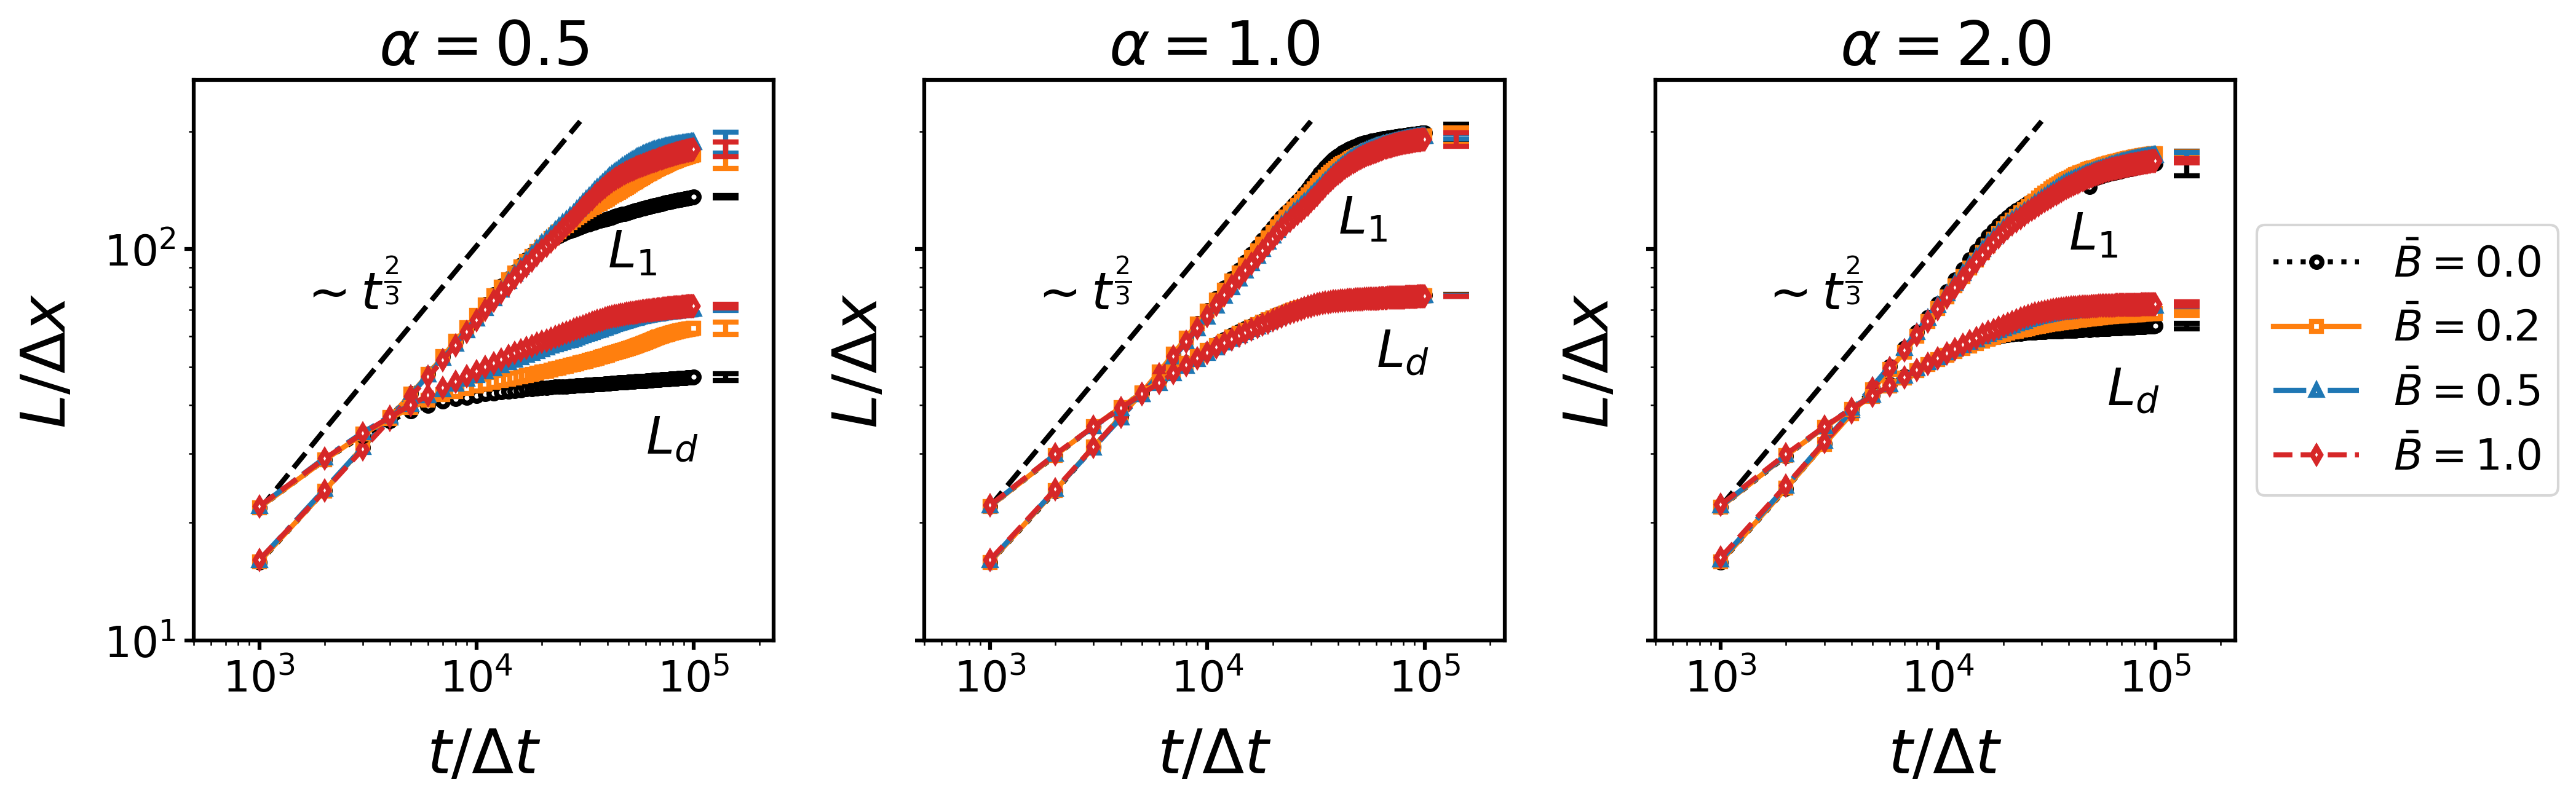
\includegraphics[width=\textwidth]{figures/results/paper1/domain_size.png}
\caption{Time dependence of the average domain size of the bijel for different particles shapes $\alpha$ and at different magnetic field strength $\bar{B}$. $L_1$ denotes the domain size obtained from the first moment of the spherical average structure factor, and $L_d$ denotes the domain size obtained from the second moment of the 3D structure factor. The increase roughly follows a $\sim t^{2/3}$ scaling law indicative of the inertial regime of spinodal decomposition.}
\label{fig:domain_size}
\end{figure*}

\subsection{Effect of magnetic field on bijel formation}

\begin{figure}
\centering
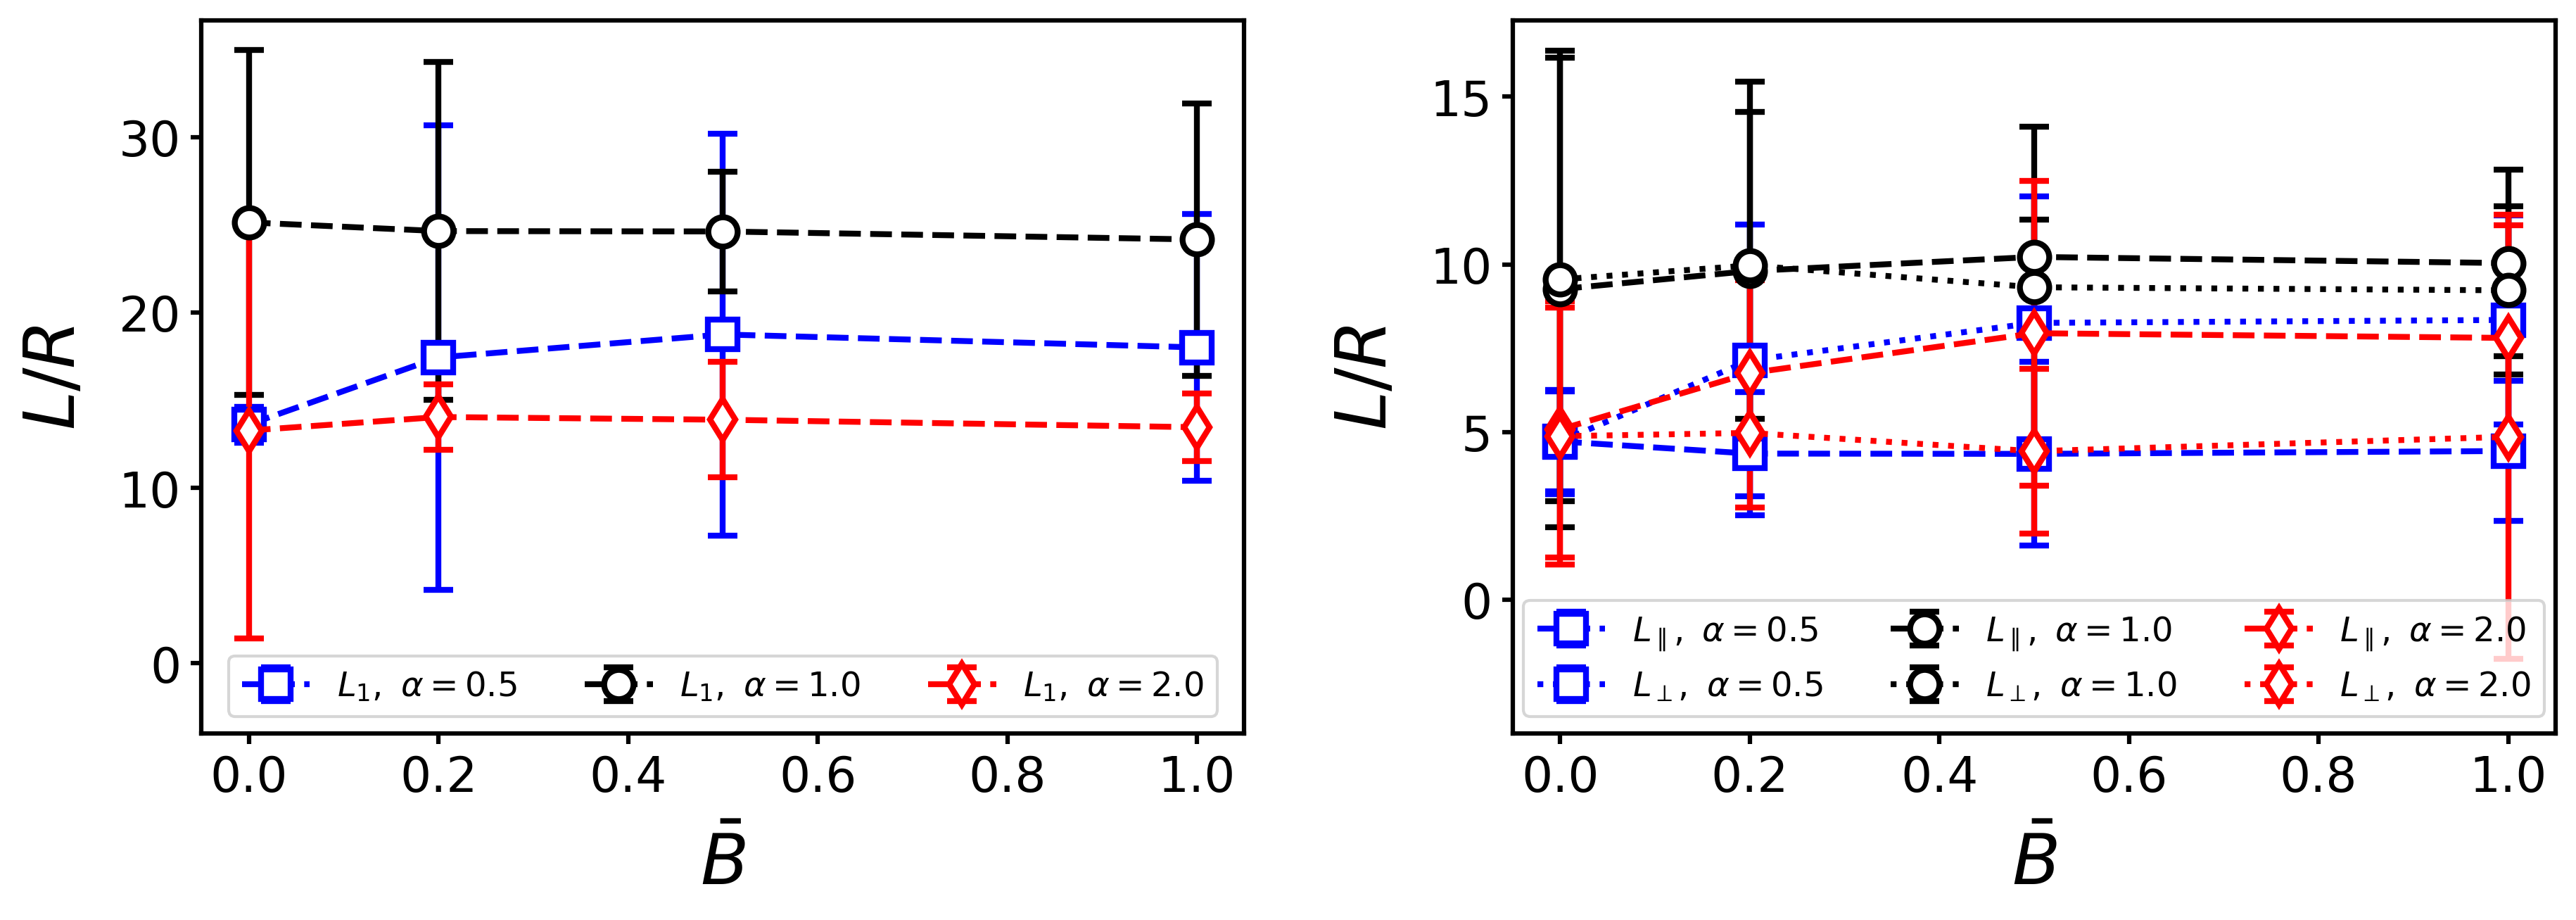
\includegraphics[width=\columnwidth]{figures/results/paper1/D2a-vs-B_ss.png}
\caption{Dependence of the average domain size on the magnetic field strength $\bar{B}$. The left plot shows the average domain size $L_1$ obtained from the spherically averaged structure factor. The right plot shows the parallel and perpendicular domain size obtained from the respective second moments of the 3D structure factor. Errorbars indicate the standard deviation taken over three independent simulation runs. For anisotropic particles, the directional domain size becomes more anisotropic with increasing field strength.}
\label{fig:D2a_B}
\end{figure}

At first glance, the time-dependence of the domain size in Fig.
\ref{fig:domain_size} suggests that the domain size is not strongly
affected by the external magnetic field. In Fig.\ref{fig:D2a_B}a) we
plotted the domain size measure \(L_d\) normalized by \(R\), the larger
of the two radii of the ellipsoidal particles. The data points represent
the domain size measured at the final time step and averaged over three
independent simulation runs with the same parameters. The normalization
with the particle radius makes it apparent that the ellipsoidal
particles reduce the domain size of bijels. This observation is in line
with observations by Günther et al.~\cite{gunther_timescales_2014} and
indicates that -- relative to their volume -- ellipsoidal particles
stabilize a larger interface area than spherical particles. This is due
to the larger cross-sectional area of ellipsoidal particles at the same
volume. Furthermore, steric constraints prevent anisotropic particles to
pack less densely in the interface than spherical particles, as we will
discuss in more detail below.

The magnetic field does have an effect on the directional
domain size as shown in Figure \ref{fig:D2a_B} where we plotted the
domain size in the direction parallel and perpendicular to \(\vec{B}\)
separately. We find that for prolate particles, the domain size in the
parallel direction increases with the field strength up to approximately
three particle radii for the largest field, while the perpendicular
domain size stays constant. This trend is reversed for oblate particles
for which the domain size in the parallel direction decreases slightly
with field strength while the perpendicular domain size increases by
approximately four particle radii. Without a field, prolate
particles lead to smaller domain size than both spherical and oblate
particles, whereas they increase the domain size when the bijel forms under the
influence of a magnetic field. The anisotropy is due to the alignment of
ellipsoidal particles which leads to a closer packing within the
interface akin to nematic ordering. The difference between oblate and
prolate particles is caused by the orientation of the magnetic dipole
moment \(\vec{m}\) along the symmetry axis of the particles. In our
model, \(\vec{m}\) is aligned with the larger axis of prolate
ellipsoids, whereas it is aligned with the smaller axis of oblate
ellipsoids. Hence \(\vec{m}\) lies in the plane of the larger
cross-section of prolate particles while \(\vec{m}\) is perpendicular to
the larger cross-section of oblate particles. We thus expect that
alignment of the particles with the magnetic field \(\vec{B}\)
facilitates closer packing perpendicular to the field for prolate
particles, and parallel to the field for oblate particles. The
increase/decrease of domain size levels off at intermediate field
strength and further increases of the field have no additional effect.

\subsection{Tortuosity}

\begin{figure*}
\centering
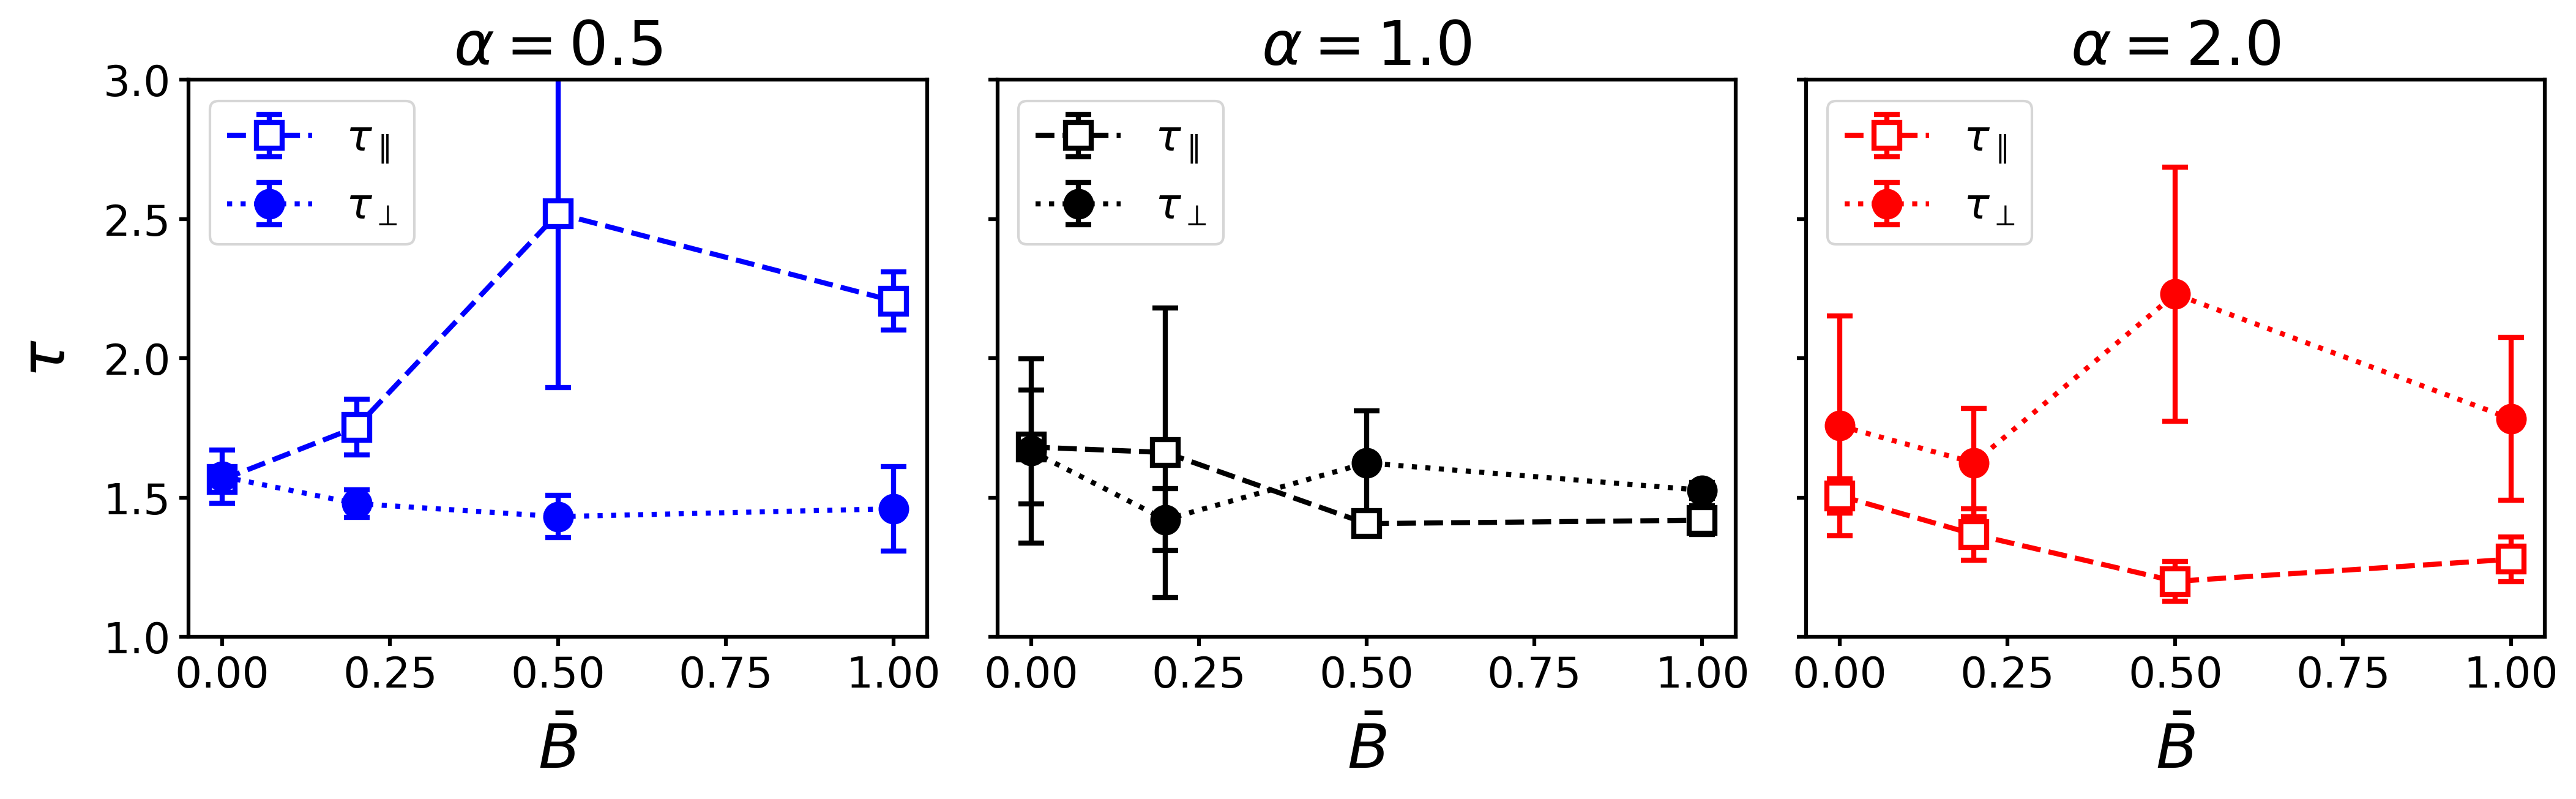
\includegraphics[width=\textwidth]{figures/results/paper1/tortuosity_compare.png}
\caption{Dependence of the tortuosity on the magnetic field strength $\bar{B}$ for different particle shapes $\alpha$. Different components of the tortuosity tensor show the anisotropy for oblate and prolate particles.}
\label{fig:tau_B}
\end{figure*}

The anisotropy of domain size suggests that the magnetic field
influences the bijel morphology at the microscale. To investigate
whether these structural changes have an effect on macroscopic
transport properties, we also characterized the tortuosity of the
bijels. Various definitions of tortuosity have been proposed in the
literature \cite{dasilva_tortuosity_2022}, including geometric,
diffusional, and hydraulic tortuosity. Here we use the diffusional
tortuosity $\tau= \frac{\epsilon D}{D_{\text{eff}}}$, i.e., the ratio of the 
effective diffusivity $D_{\text{eff}}$ and the intrinsic diffusivity
$D$. Porous structures were generated from the order parameter field
at the last time step of the simulations by binarizing the raw order
parameter data using a threshold of zero. We masked the largest
connected component representing the percolating domain and then used
the Python package \texttt{taufactor}\cite{cooper_taufactor_2016} to
calculate the tortuosity in the three Cartesian coordinate
directions. \texttt{taufactor} determines the tortuosity by comparison
of steady-state diffusive flow through a porous medium with the bulk
diffusive flow in a control volume of the same size, molecular
diffusivity, and driving force \cite{cooper_taufactor_2016}. We used
the \texttt{PeriodicSolver} to employ periodic boundary conditions.

Figure \ref{fig:tau_B} shows the results for the tortuosity as a
function of the applied magnetic flux for the three particle aspect
ratios. In the absence a magnetic field, the three aspect ratios lead to
a similar tortuosity around $\tau\approx 1.5$, slightly larger than
the tortuosity predicted by the Bruggeman relation
\(\tau=\epsilon^{-0.5}=1.41\) for equal volume fractions
\(\epsilon=0.5\) of the phases
\cite{bruggeman1935tortuosity, tjaden_origin_2016}. The observed
tortuosity is consistent with simulations of gyroid structures by Luo et
al., who found diffusive tortuosities in the range from 1.48 to 1.73
\cite{luo_macroscopic_2020}. Figure \ref{fig:tau_B} shows that in an
applied magnetic field, the tortuosity of bijels stabilized by
anisotropic particles (\(\alpha\neq1\)) becomes anisotropic as well.
Oblate particles (\(\alpha=0.5\)) lead to an increase of the tortuosity
\(\tau_\parallel\) in the direction of the magnetic field while the
tortuosity in the direction perpendicular to the magnetic field remains
around \(\tau_\parallel\approx1.5\). Conversely, prolate particles
(\(\alpha=2\)) lead to an increase of the tortuosity in the direction
perpendicular to the magnetic field, while the tortuosity in the
parallel direction slightly decreases with increasing field strength. In
both cases, the changes in tortuosity are consistent with the
anisotropic domain size and the alignment of particles with the magnetic
field. For prolate particles, the longer axis is aligned with the
magnetic moment and induces larger domain size and lower tortuosity in
this direction. The results show that the magnetic field has a
noticeable effect on the tortuosity of the bijel. We observe that the
largest change of tortuosity is measured at intermediate field strength
\(\bar{B}=0.5\). This suggests that the competition of interfacial and
magnetic forces and the resulting alignment of particles and liquid
domains induces morphological changes that are more complex than a
monotonic increase or decrease. We therefore turn to investigate the
microstructural changes within the bijel morphology in more detail.

\subsection{Kinetics of bijel formation in magnetic fields}

To shed light on the mechanisms involved in the coarsening dynamics,
we now turn to the kinetics of bijel formation in more detail. The
coarsening dynamics can be characterized by a coarsening speed. Here,
we use the finite difference of the directional domain size to
calculate the components of the coarsening velocity
%
\begin{equation}
u_{L_\beta}(t) = \frac{L_\beta(t+\Delta t_s)-L_\beta(t-\Delta t_s)}{2\Delta t_s} ,
\end{equation}
%
where \(\Delta t_s\) is the time between simulation
snapshots, and $\beta$ denotes either the direction parallel or perpendicular to the magnetic field.

\begin{figure*}
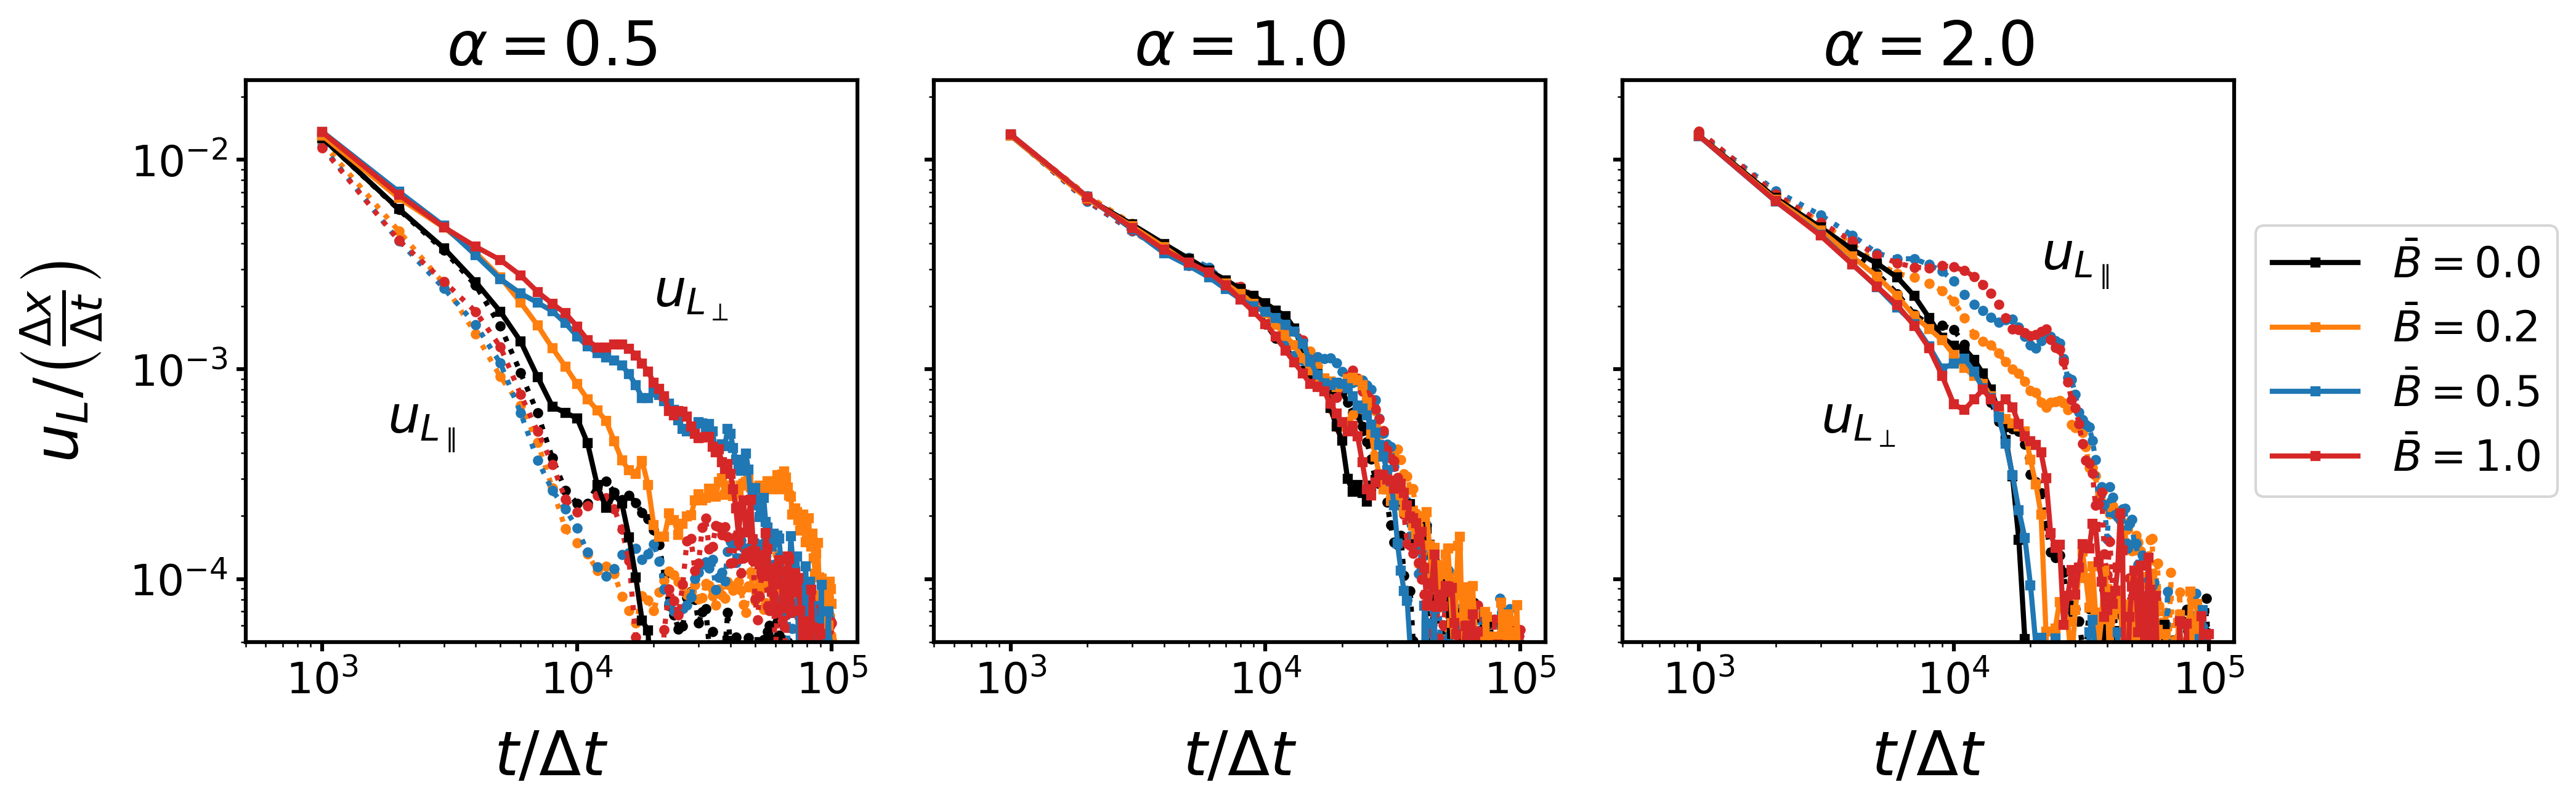
\includegraphics[width=\textwidth]{figures/results/paper1/coarsening_vel.png}
\caption{Time-dependence of the coarsening velocity $u_L$ for different particles shapes $\alpha$  and at different magnetic field strength $\bar{B}$. The different components of the coarsening velocity show that the jamming time is different in the direction parallel and perpendicular to the magnetic field.}
\label{fig:coarsening_velocity}
\end{figure*}

Figure \ref{fig:coarsening_velocity} shows the coarsening speed in the directions parallel and perpendicular to the applied magnetic field. The data confirms that for spherical particles, domain coarsening remains isotropic. We observe a higher coarsening speed initially which slows at later times when the particles begin to jam. This indicates that the
coarsening is subject to different time scales, as reported previously
by Harting and co-workers \cite{gunther_timescales_2014}. Reeves et
al.~\cite{reeves_particle-size_2015} have pointed out that bijel
formation hinges on the jamming time in relation to the disruption time, i.e., the time scale at which domain pinch-off events can cause bijel break-up through depercolation. In our simulations, however, we have not observed disruption of bijel formation; stable bijels form for all parameters consistent with simulations by Stratford et
al.~\cite{stratford_colloidal_2005} and Jansen et al.~\cite{jansen_bijels_2011}.

For ellipsoidal particles, our data clearly shows that an\-isotropic
domain coarsening arises in magnetic fields.  For oblate particles
(\(\alpha=0.5\)), the coarsening speed in the direction perpendicular
to the field increases with increasing magnetic field strength.
Jamming in this direction appears to be delayed compared with the
direction parallel to the field. The coarsening speed in the parallel
direction remains comparable to the case without an applied magnetic
field. This anisotropic behavior of the coarsening speed reverses for
prolate particles, where the coarsening speed in the direction parallel to the field increases with increasing field strength, and jamming in this direction
is delayed compared with the perpendicular direction. In addition, we observe a shoulder (around \(10^4\Delta t\)) where the coarsening speed decays more slowly before jamming sets in. These results suggest that the coarsening near the jamming time is affected by a mechanism that depends on the applied magnetic field and causes the anisotropic
behavior. This mechanisms involves the re-orientation of anisotropic
particles and their alignment relative to the direction of the
magnetic field. To confirm this hypothesis, we analyze the
orientational order of the particles and their alignment relative to
the magnetic field and the interface, respectively.

\subsection{Particle re-orientation and packing}

\begin{figure}
\centering
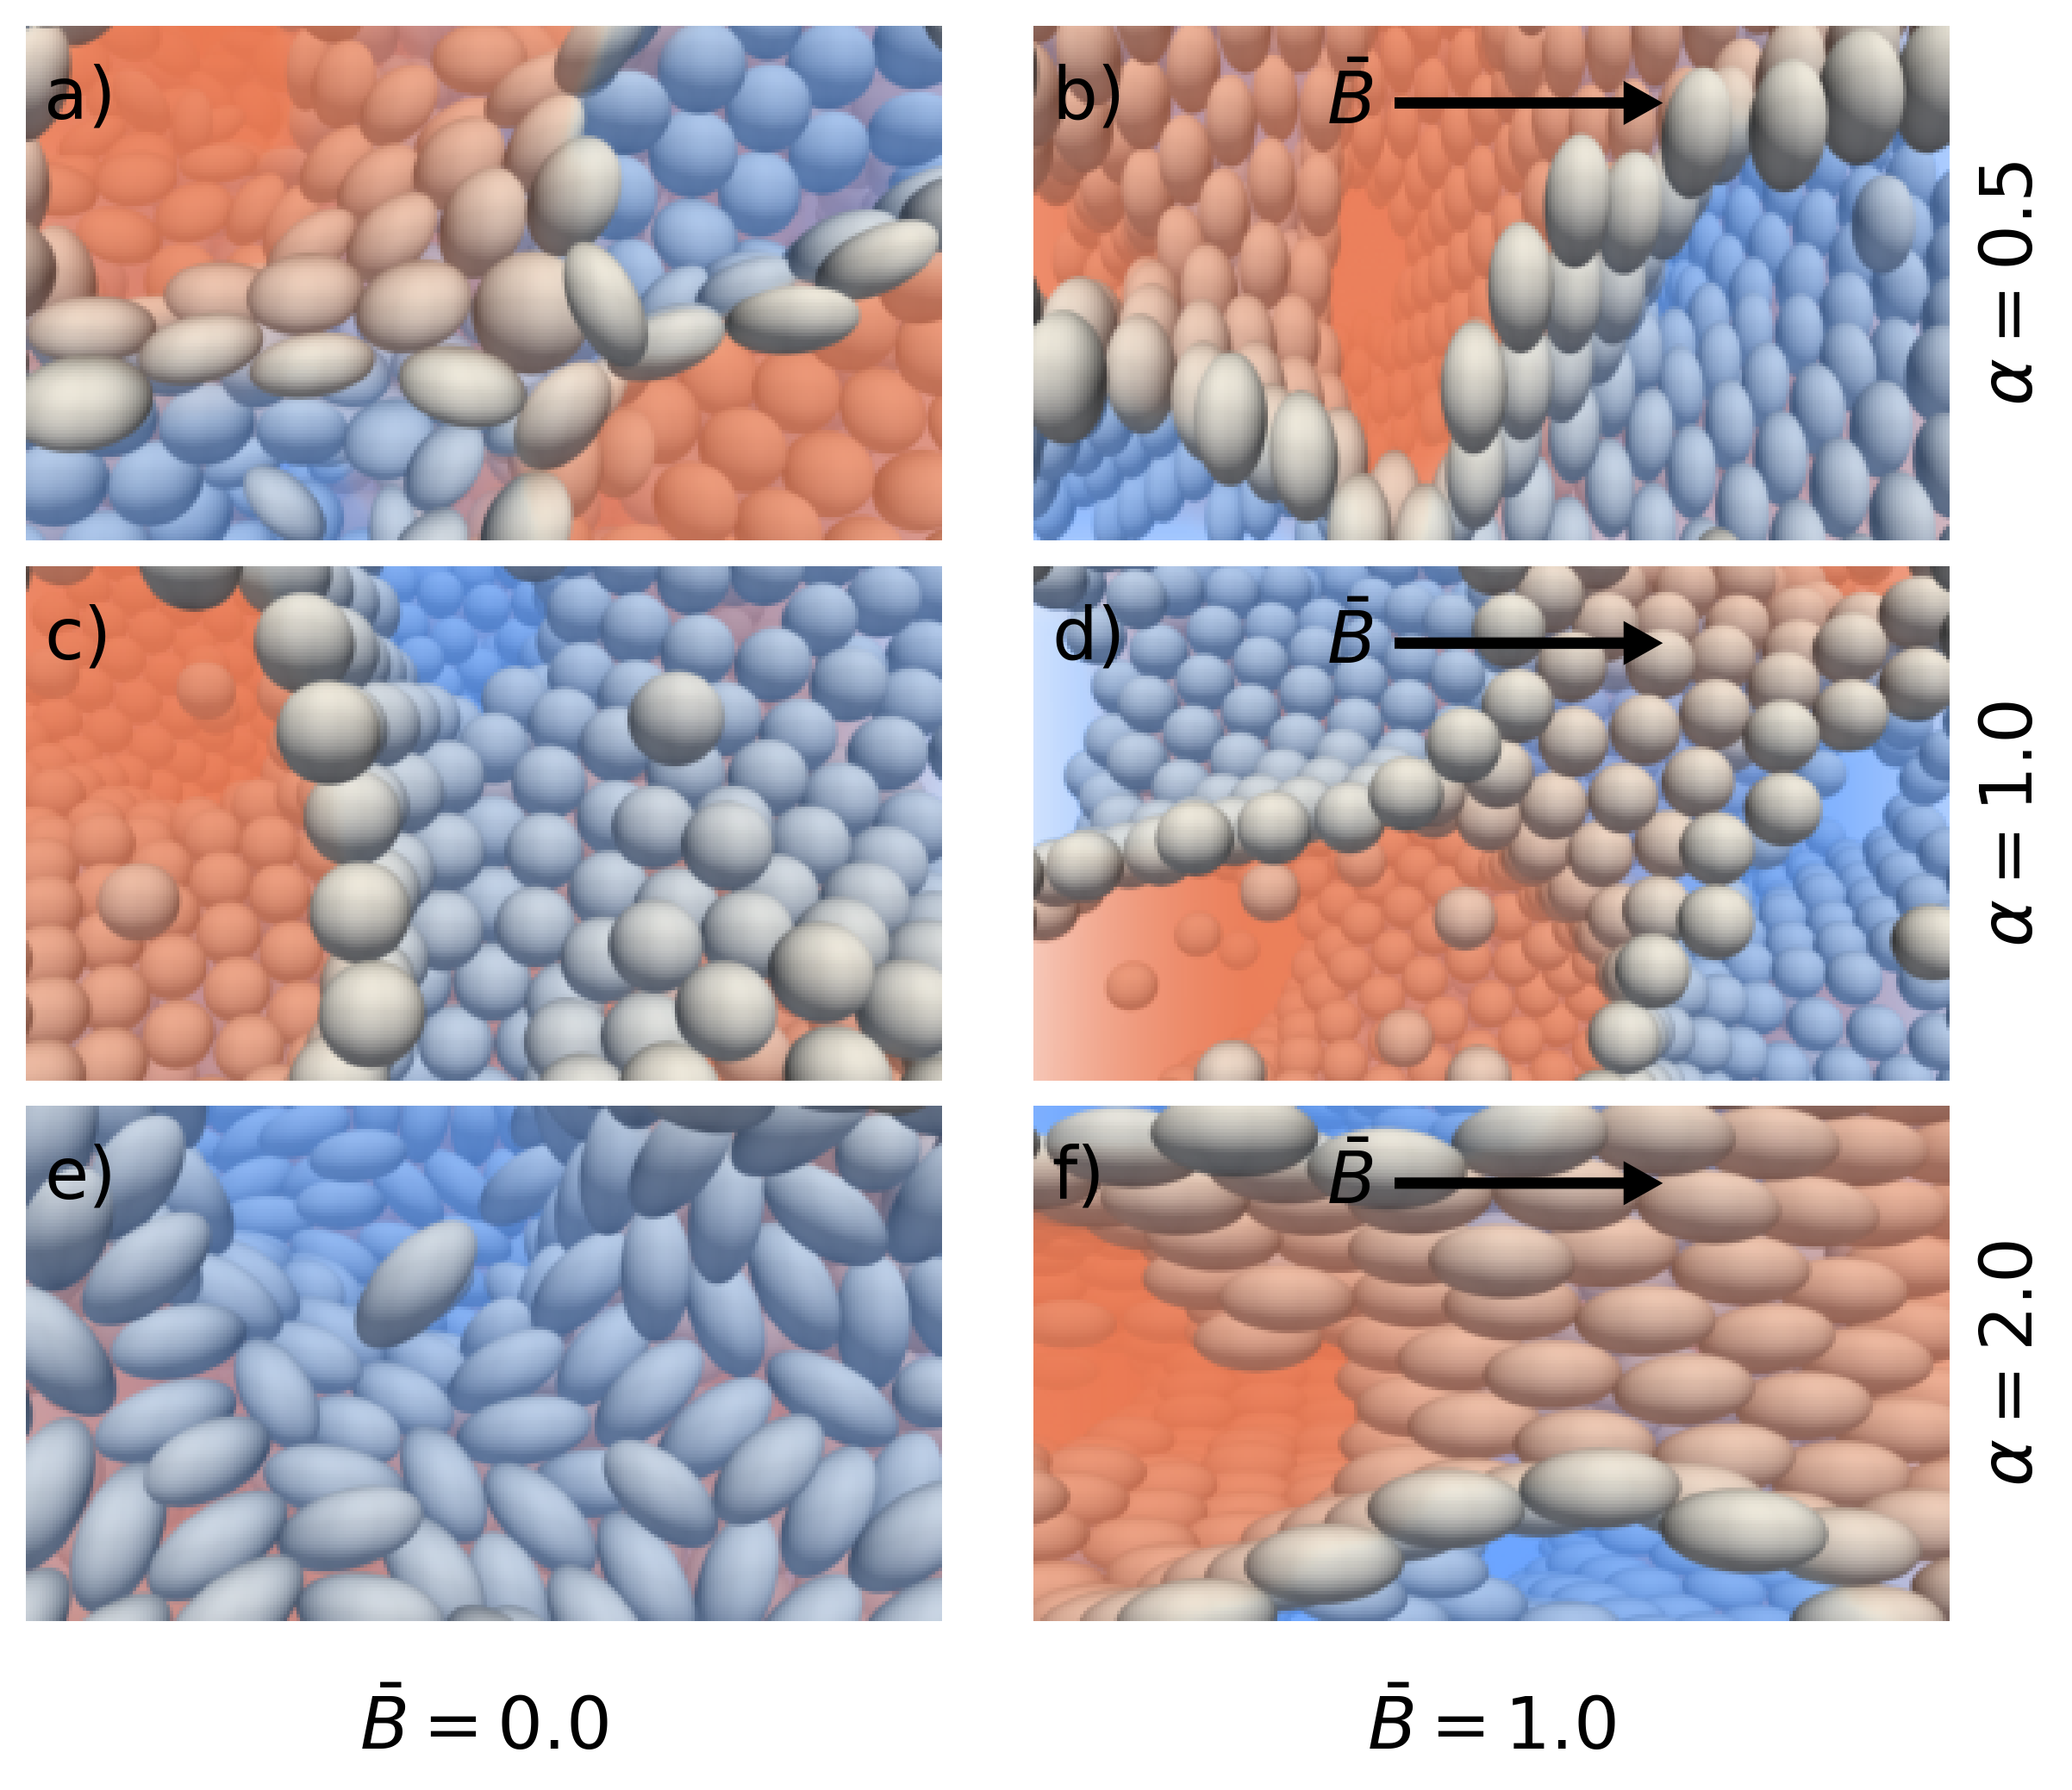
\includegraphics[width=\columnwidth]{figures/results/paper1/particle_packing_viz.png}
\caption{Snapshots illustrating the particle packing at the interface for different particle shapes $\alpha$ with (left) and without (right) applied magnetic field $\bar{B}$. The right column shows the alignment of the symmetry axis of the oblate (top row) and prolate (bottom row) particles in the direction of the magnetic field indicated by arrows.}
\label{fig:packing_viz}
\end{figure}

The primary effect of the magnetic field is the torque it exerts on the
magnetic dipole of the particles. This torque rotates the particles
towards the direction of the magnetic field. The alignment of the
particles with the field direction can be clearly observed in the
simulation snapshots shown in Figure \ref{fig:packing_viz}. While the
particles are oriented randomly in the interface in the absence of a
magnetic field (\(\bar{B}=0\)), the magnetic field induces orientational
order of the magnetic dipoles (shown for \(\bar{B}=1\)).

\begin{figure}
\centering
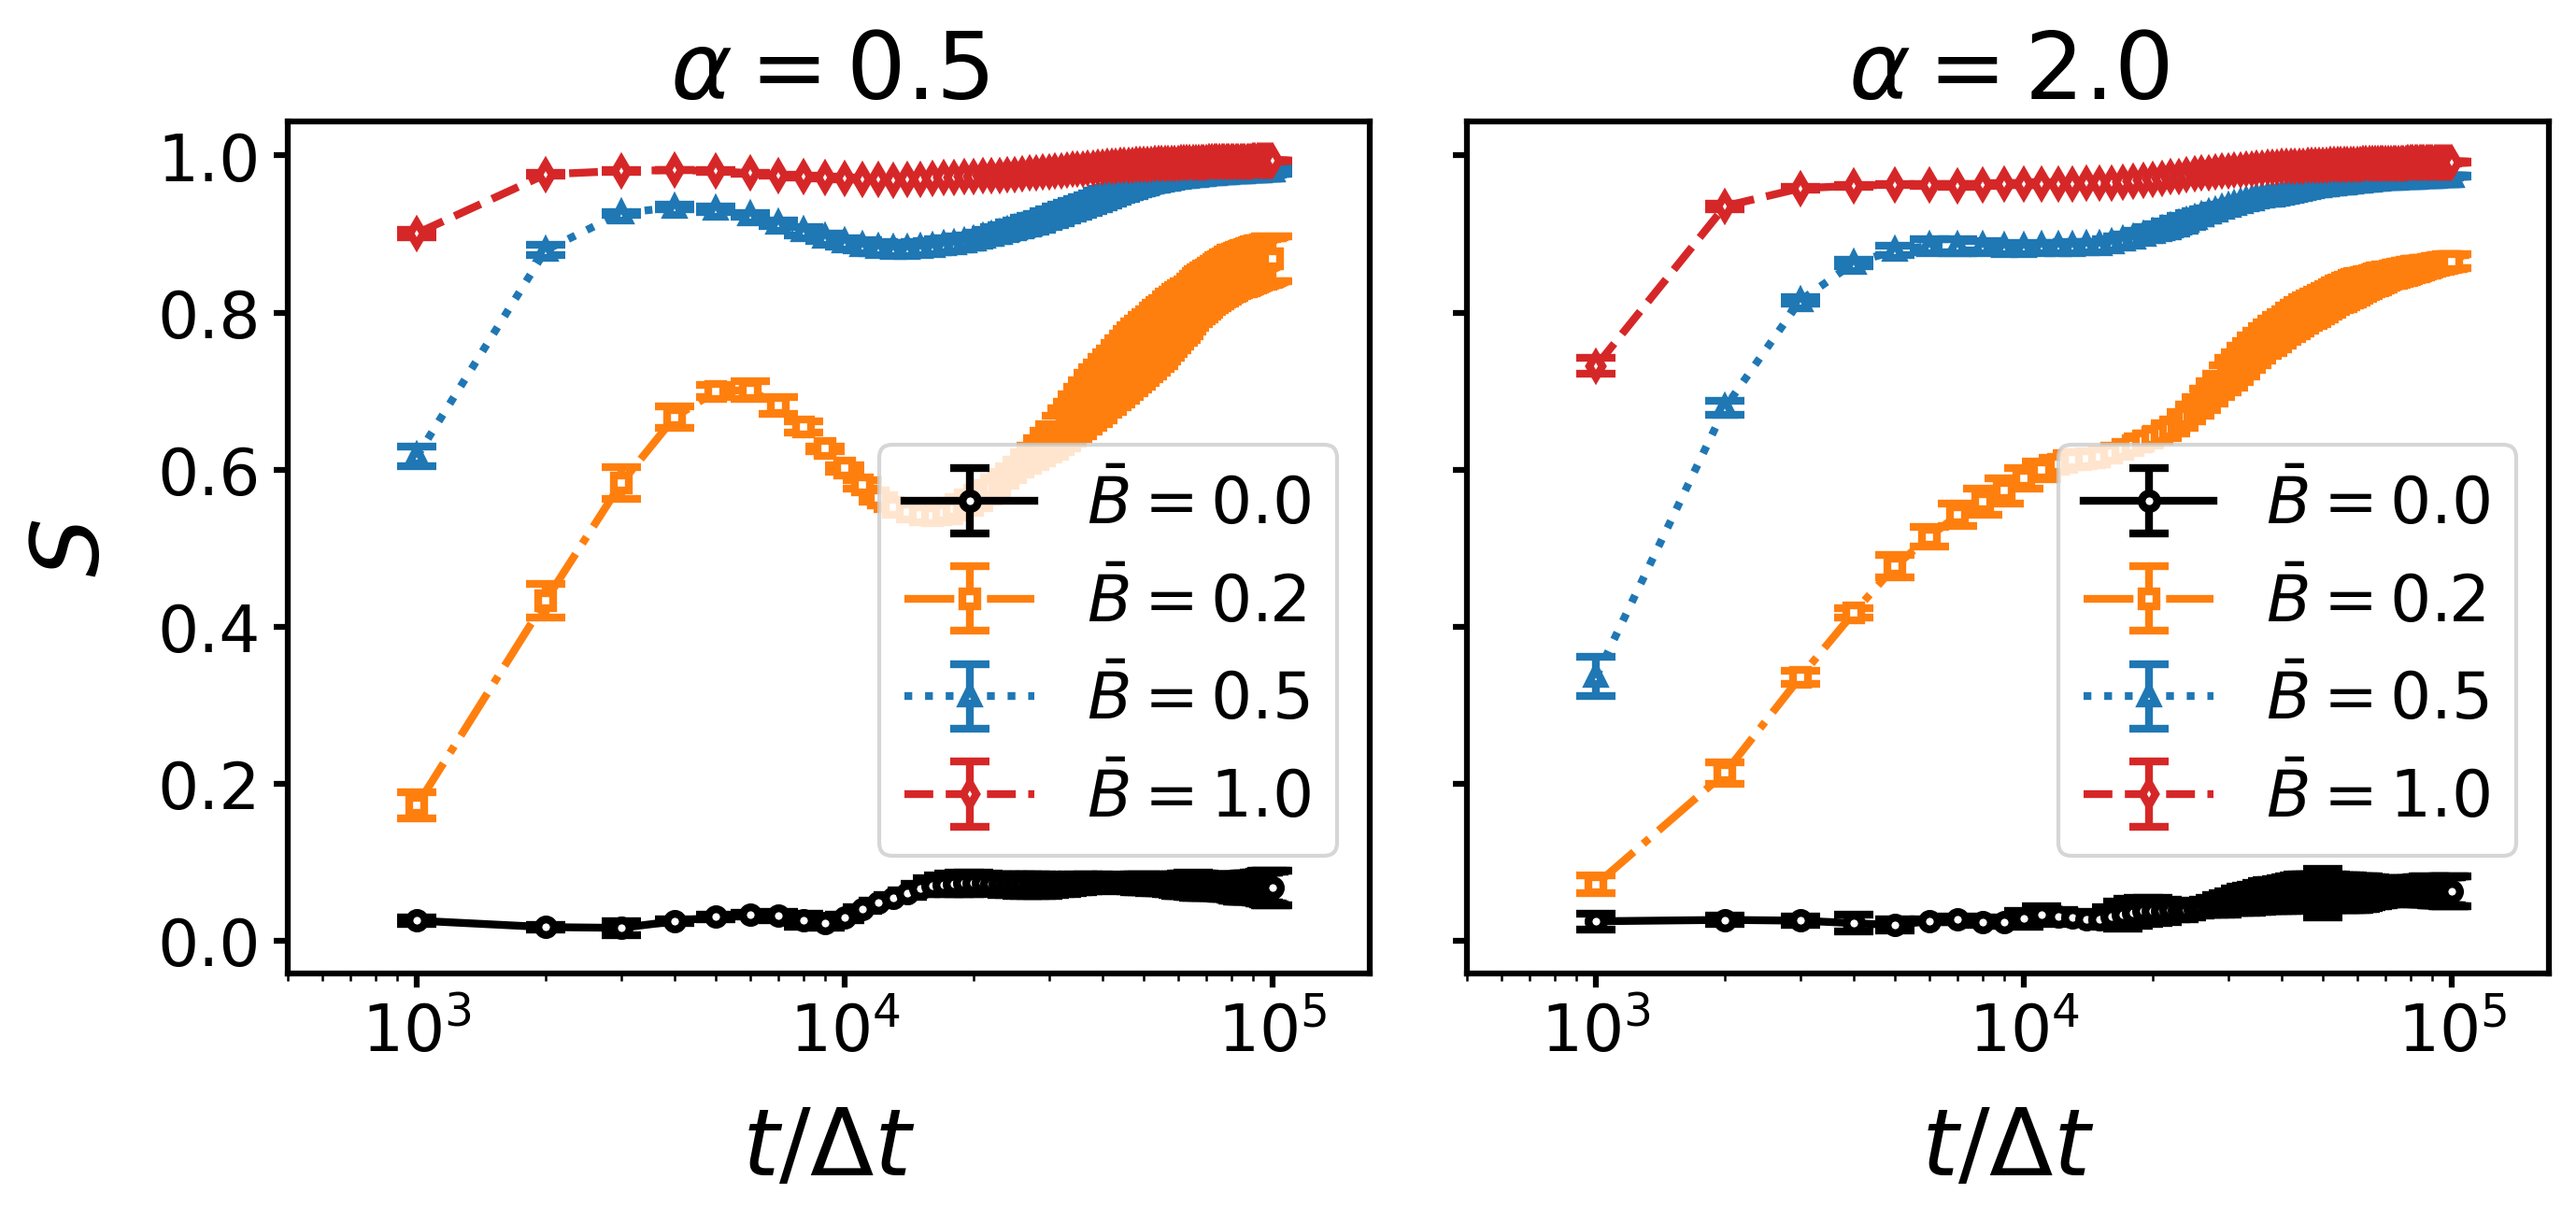
\includegraphics[width=\columnwidth]{figures/results/paper1/S-vs-t.png}
\caption{Time-dependence of the nematic order parameter $S$ of oblate ($\alpha=0.5$) and prolate ($\alpha=2$) particles at different field strength $\bar{B}$. Errorbars indicate the standard deviation taken over three independent simulation runs. Nematic order generally increases with applied field strength for all particle geometries. The increase slows down (for prolate particles) or reverses (for oblate particles) around $10^4$ timesteps.}
\label{fig:nematic_time}
\end{figure}

To measure the particle alignment quantitatively, we computed the
nematic order tensor \cite{veerman_phase_1992}
%
\begin{equation}
\tens{Q} = \frac{1}{n_p} \sum_i \left( \frac{3}{2} \hat{\vec{o}}_i \otimes \hat{\vec{o}}_i -\frac{1}{2}\mathsf{1} \right)
\end{equation}
%
where \(\hat{\vec{o}}_i\) is the orientation of the
\(i\)-th particles and \(n_p\) is the number of particles in the system.
The largest eigenvalue of $\tens{Q}$ yields the nematic order
parameter
%
\begin{equation}
S = \left\langle \frac{3}{2}\cos^2 (\theta) - \frac{1}{2} \right\rangle ,
\end{equation}
%
where
\(\theta=\arccos(\hat{\vec{o}}_i\cdot\hat{\vec{n}})\) is the angle
between the particle orientation and the nematic director
\(\hat{\vec{n}}\).

Figure \ref{fig:nematic_time} shows the time evolution of the nematic
order parameter \(S\) for the three different particle aspect ratios
\(\alpha\) and varying magnetic field strength \(\bar{B}\). The onset of
orientational order is nearly instantaneous and increases with
increasing field strength. For magnetic flux densities
\(\bar{B}\ge0.5\), the nematic order parameter saturates at
\(S\approx 1.0\) towards the end of the simulation. For the prolate
particles (\(\alpha=2.0\)), we observe a shoulder at around
\(10^4\Delta t\) and an intermittent plateau. The occurrence of this
plateau coincides with the slowed decay of the coarsening speed in Fig.
\ref{fig:coarsening_velocity}. This change in the orientational ordering
is even more distinct for the oblate particles, where the nematic order
decays intermittently before it increases again. The intermittent decay
for oblate particles, and the plateau for prolate particles, correlate
with the delayed onset of jamming in the direction perpendicular and
parallel to the magnetic field, respectively. These observations can be
interpreted as follows: The magnetic field aligns the particles with the
direction of the magnetic field early during the simulation. Due to this
alignment, the steric constraints between particles adsorbed at the
interface are reduced which allows further coarsening of the interfacial
area. However, during coarsening, the interfaces may re-orient
themselves and cause a capillary torque on the particles that competes
with the magnetic torque. This competition intermittently perturbs the
nematic order of the particles leading to the observed decay and plateau
of the nematic order parameter. Accordingly, the decay of \(S\) is most
pronounced at the weakest magnetic field \(\bar{B}=0.2\).

To further corroborate this mechanism, we quantify the orientational
order of the interfaces. We computed the interfacial orientation tensor
%
\begin{equation}
\tens{Q}_{\text{int}} = \frac{1}{\langle \mathrm{tr}(\tens{A}) \rangle} 
\left\langle \tens{A} - \frac{1}{3} \mathrm{tr}(\tens{A}) \mathsf{1} \right\rangle ,
\end{equation}
%
where the local tensor field $\tens{A}$ is defined by
%
\begin{equation}
\tens{A} = \nabla\phi\otimes\nabla\phi .
\end{equation}
%
The largest eigenvalue of $\tens{Q}$ is taken as the
interface nematic order parameter $S_{\text{int}}$.

\begin{figure}
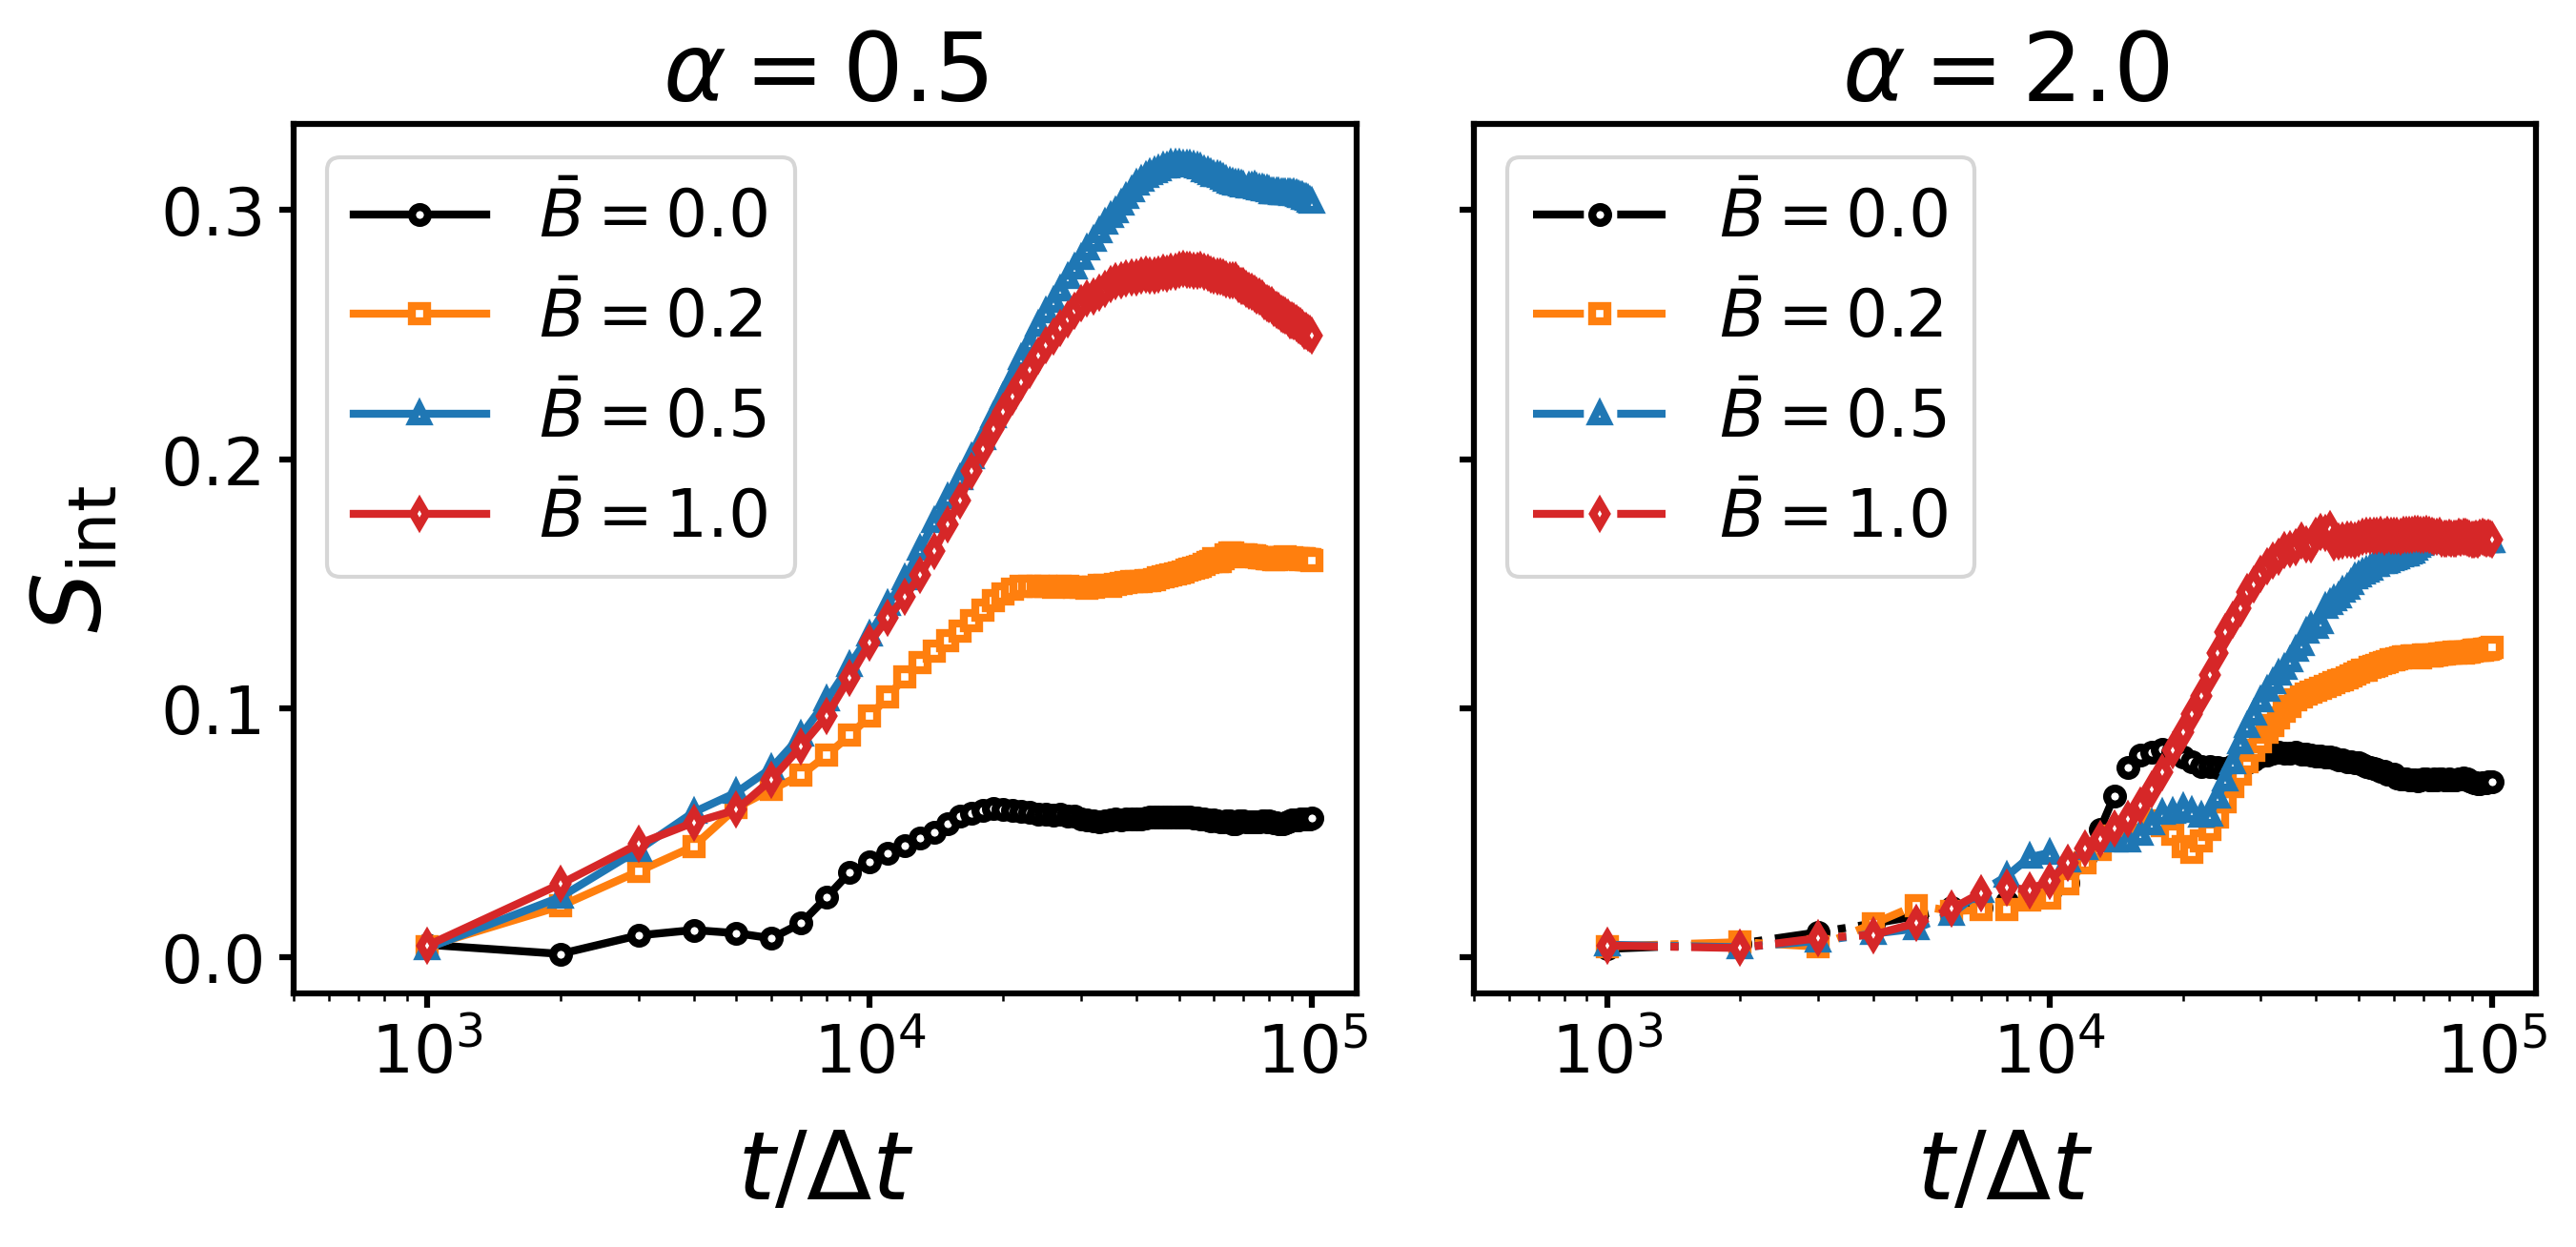
\includegraphics[width=\columnwidth]{figures/results/paper1/interface_nematic.png}
\caption{Time-dependence of the interface nematic order for oblate ($\alpha=0.5$) and prolate ($\alpha=2$) particles at different magnetic field strength $\bar{B}$. The interface alignment tends to increase with increasing field strength. The rate of increase becomes larger around $10^4$ timesteps, indicating the alignment of the interfaces due to capillary interactions with the particles.}
\label{fig:interface_nematic}
\end{figure}

The results for the interface nematic order parameter $S_{\text{int}}$
are shown in Figure \ref{fig:interface_nematic}. The nematic interface
alignment increases over time and the rate of increase appears to be
higher for larger magnetic field strength $\bar{B}$. In all cases, the
final value of $S_{\text{int}}$ is below 0.5 indicating that the
tortuous structure of the interface is maintained in the presence of
magnetic fields. This confirms that the re-orientation of the particles
does not disrupt the bijel structure but leads to partial alignment of
the interfaces without changing the general topology of the bicontinuous
morphology.

When the particles rotate, the interface exerts a capillary torque on
the particles due to the surface tension and the contact angle. If the
magnetic torque exceeds the interfacial forces, the particles can
potentially overcome the capillary torque and rotate out of the
interface. For prolate particles (\(\alpha=2\)) adsorbed at flat
interfaces, Davies et al. have shown that a transition between the
energetically preferred ``flat'' orientation and a tilted orientation
occurs at a critical field strength of approximately \(\bar{B}=0.2\)
\cite{bresme_orientational_2007,davies_interface_2014,newton_influence_2014}.
In the case of bijels, however, the percolating interfaces are tortuous
and thus more mobile. We therefore posit that, rather than tilting out
of the interface, rotating particles can ``pull'' the interface along
and thereby align the liquid domains. For anisotropic particles, we
expect that the interfaces align along the larger cross-section of the
particles, i.e., perpendicular to the symmetry axis of oblate particles
and parallel to the symmetry axis of prolate particles. The data for the
anisotropic domain size and tortuosity above is consistent with this
assumption. To ascertain that the particles remain indeed in their
energetically preferred orientation with respect to the interface, we
analyzed the angle between the symmetry axis of the particles and the
interface normal. To this end, we generated a mesh of the interface
using a marching cubes algorithm. For each particle we identified the
mesh vertex closest to the particle's position (excluding particles
whose distance to the mesh exceeds the radius of the longer particle
axis) and computed the angle between the particle orientation vector
\(\hat{\vec{o}}_i\) and the interface normal at the closest vertex.
Figure \ref{fig:psi_time} shows the time-dependence of the average angle
\(\psi\) between the particle dipole axis and the nearest interface
normal.

\begin{figure}
\centering
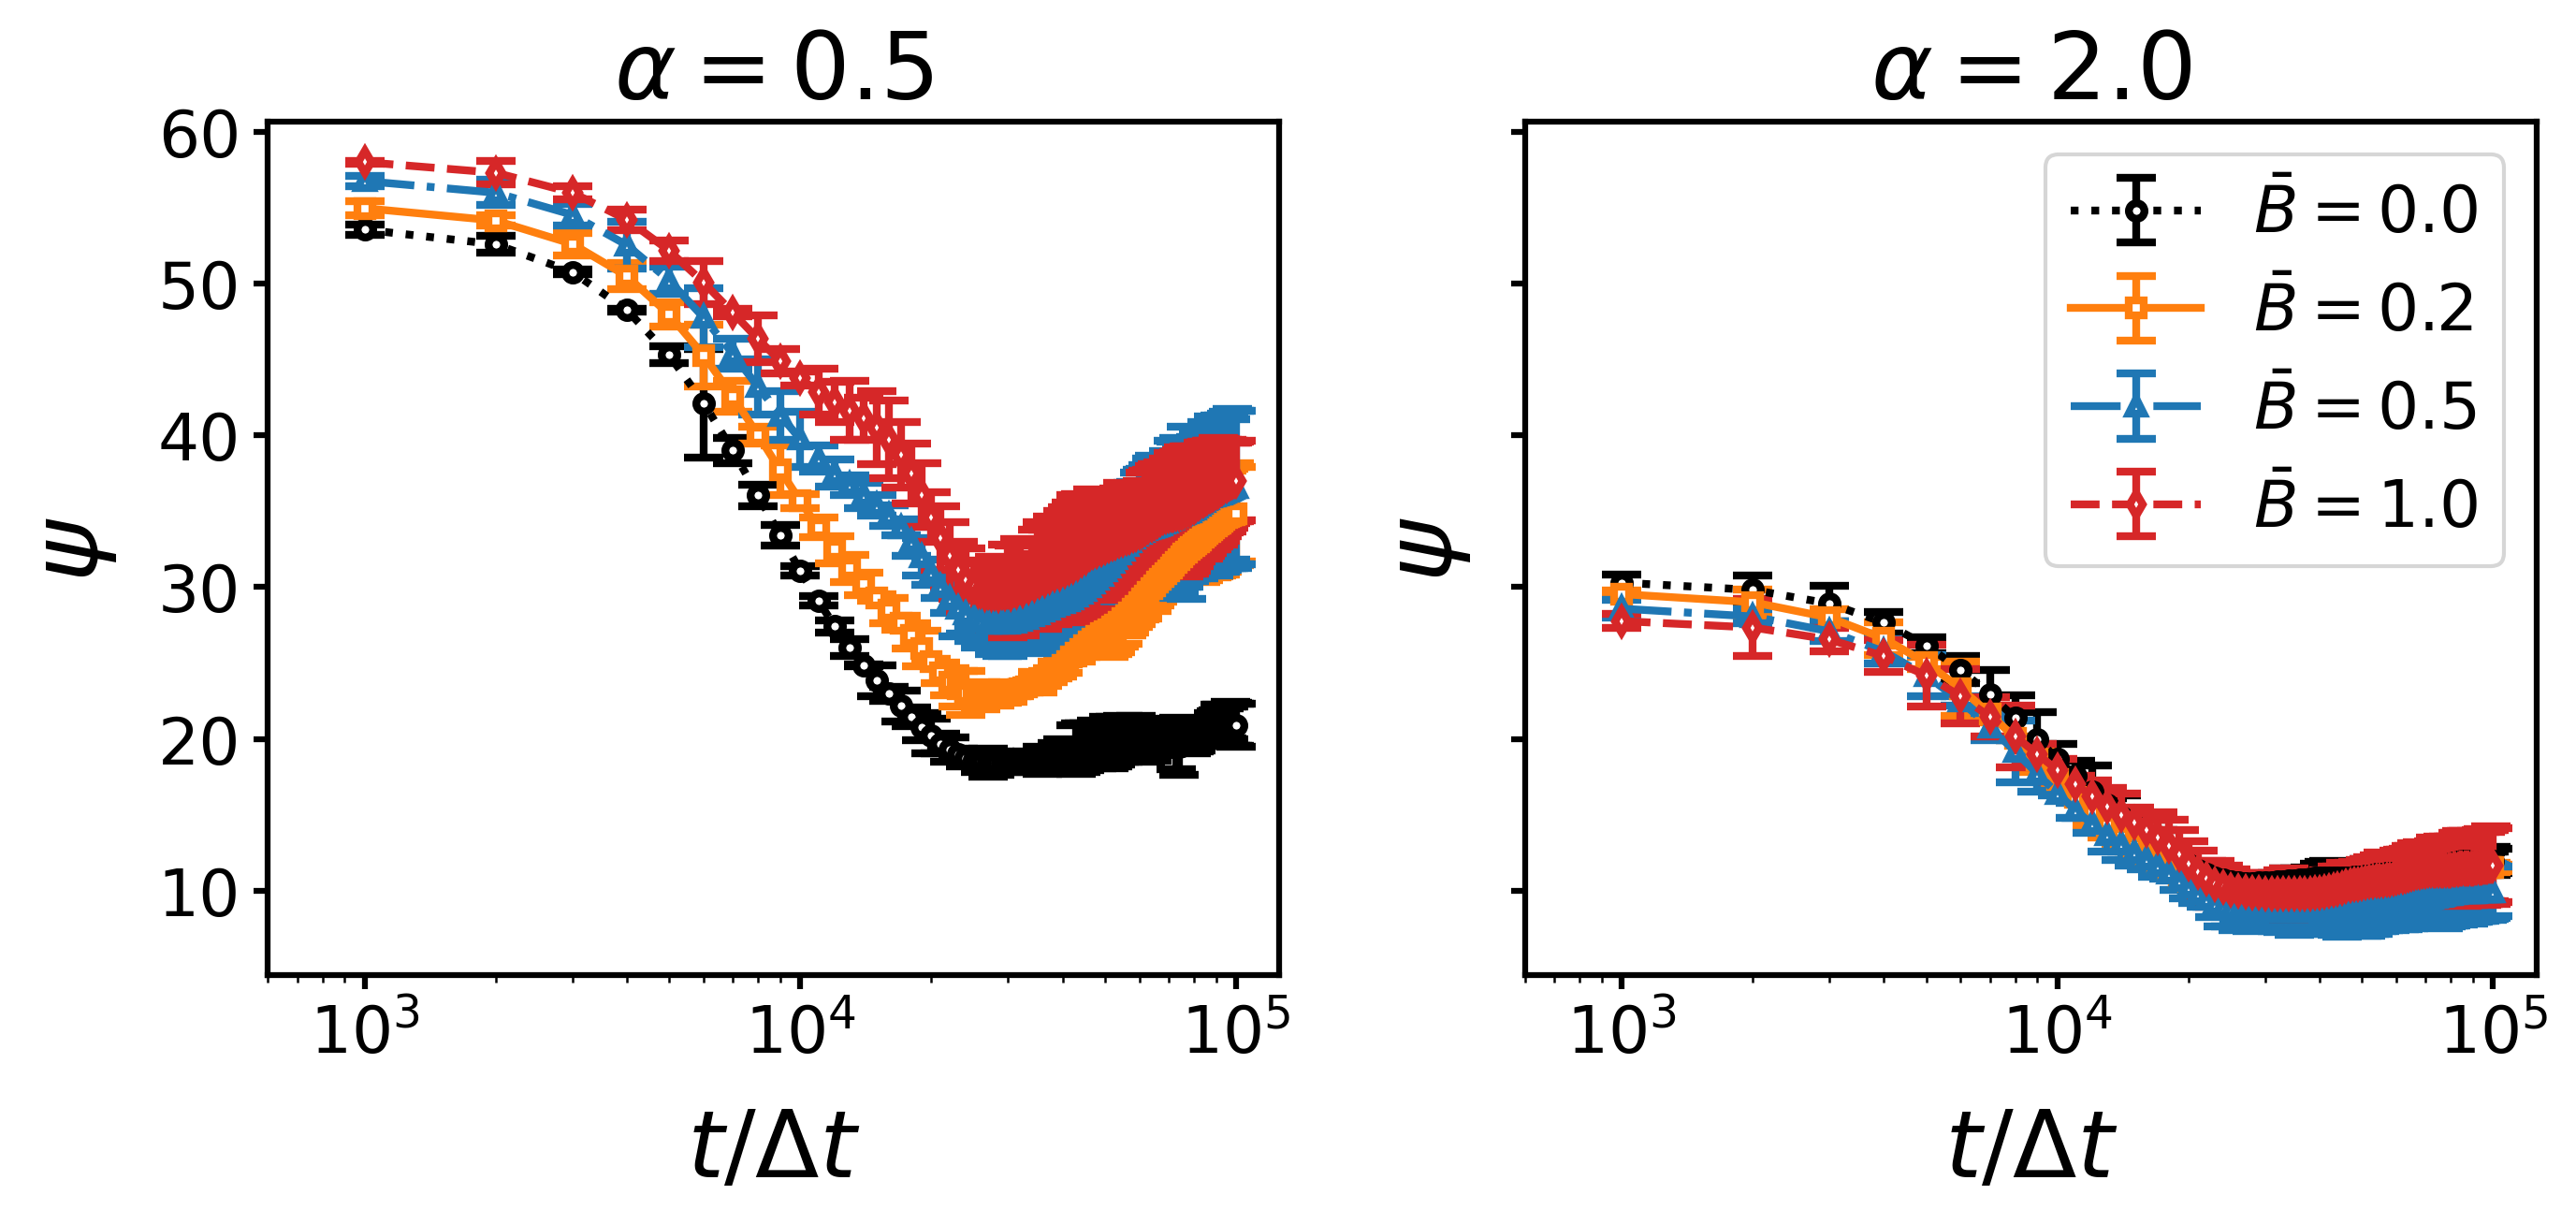
\includegraphics[width=\columnwidth]{figures/results/paper1/psi-vs-t.png}
\caption{Time-dependence of the average angle $\psi$ between the particle axis and the interface normal for oblate ($\alpha=0.5$) and prolate ($\alpha=2$) particles at different magnetic field strength $\bar{B}$. Errorbars indicate the standard deviation taken over three independent simulation runs. The angle between between the particles and the interface normal generally approaches the energetically preferred value ($0^\circ$ for oblate particls, $90^\circ$ for prolate particles). The average angle changes most rapidly around $10^4$ timesteps.}
\label{fig:psi_time}
\end{figure}

For both types of anisotropic particles, the average angle between the
particle dipole and the interface normal is initially around
\(\psi\approx60^\circ\). As the spinodal interface sweeps through the
system, particles attach to the interface and alignment due to the
capillary torque sets in. For oblate particles, the dipole axis aligns
with the interface normal as indicated by the decay of \(\psi\) towards
zero. For prolate particles, the preferential alignment of the dipole
axis is parallel to the interface and hence \(\psi\) increases towards
\(90^\circ\). The main variation of \(\psi\) occur in a time interval
around \(10^4\Delta t\) which coincides with the distinct features of
the coarsening speed and the particle nematic order observed above. The
results thus substantiate the proposed mechanism of particle
re-orientation in the magnetic field and the concomitant local alignment
of the interface. Once the particles start jamming, the shrinking
interfacial area forces some particles out of their preferred alignment
with the interface, leading to an increase of \(\psi\) for oblate
particles and a decrease of \(\psi\) for prolate particles. Figure
\ref{fig:psi_time} suggests that the forced tilting is more pronounced
for oblate particles than for prolate particles. Due to the larger
aspect ratio, the tilting of prolate particles relative to the interface
induces deformations that appear to cause a larger capillary torque than
the tilting of oblate particles. %For oblate particles, the liquid-solid
%contact line is on average further away from the particle center than
%for prolate particles, hence the lever effect of oblate particles is
%weaker and allows larger tilting relative to the the preferred alignment
%with the interface.
Hence the prolate particles remain mostly aligned with the interface
even in the stronger applied magnetic fields.

As hypothesized above, the alignment of the particle dipole axis with
the magnetic field reduces the steric constraints within the interface.
To corroborate this idea, we analyzed the radial distribution function
(RDF) of the particles
%
\begin{equation}
g(r) = \frac{n_p-1}{n_p} V \left\langle\delta\left(r-r_i\right)\right\rangle ,
\end{equation}
%
where \(n_p\) is the number of particles in the volume
\(V\), and \(\langle\cdot\rangle\) denotes an average over all
particles. The radial distribution function was calculated by binning
the distance between all particle pairs and normalizing the shells with
respect to the distribution \(4\pi \rho r^2 \mathrm{d}r\) of an ideal
gas. The time-evolution of the RDFs for the three particle shapes and
varying magnetic flux density is illustrated in Figure \ref{fig:rdf}.

\begin{figure*}
\centering
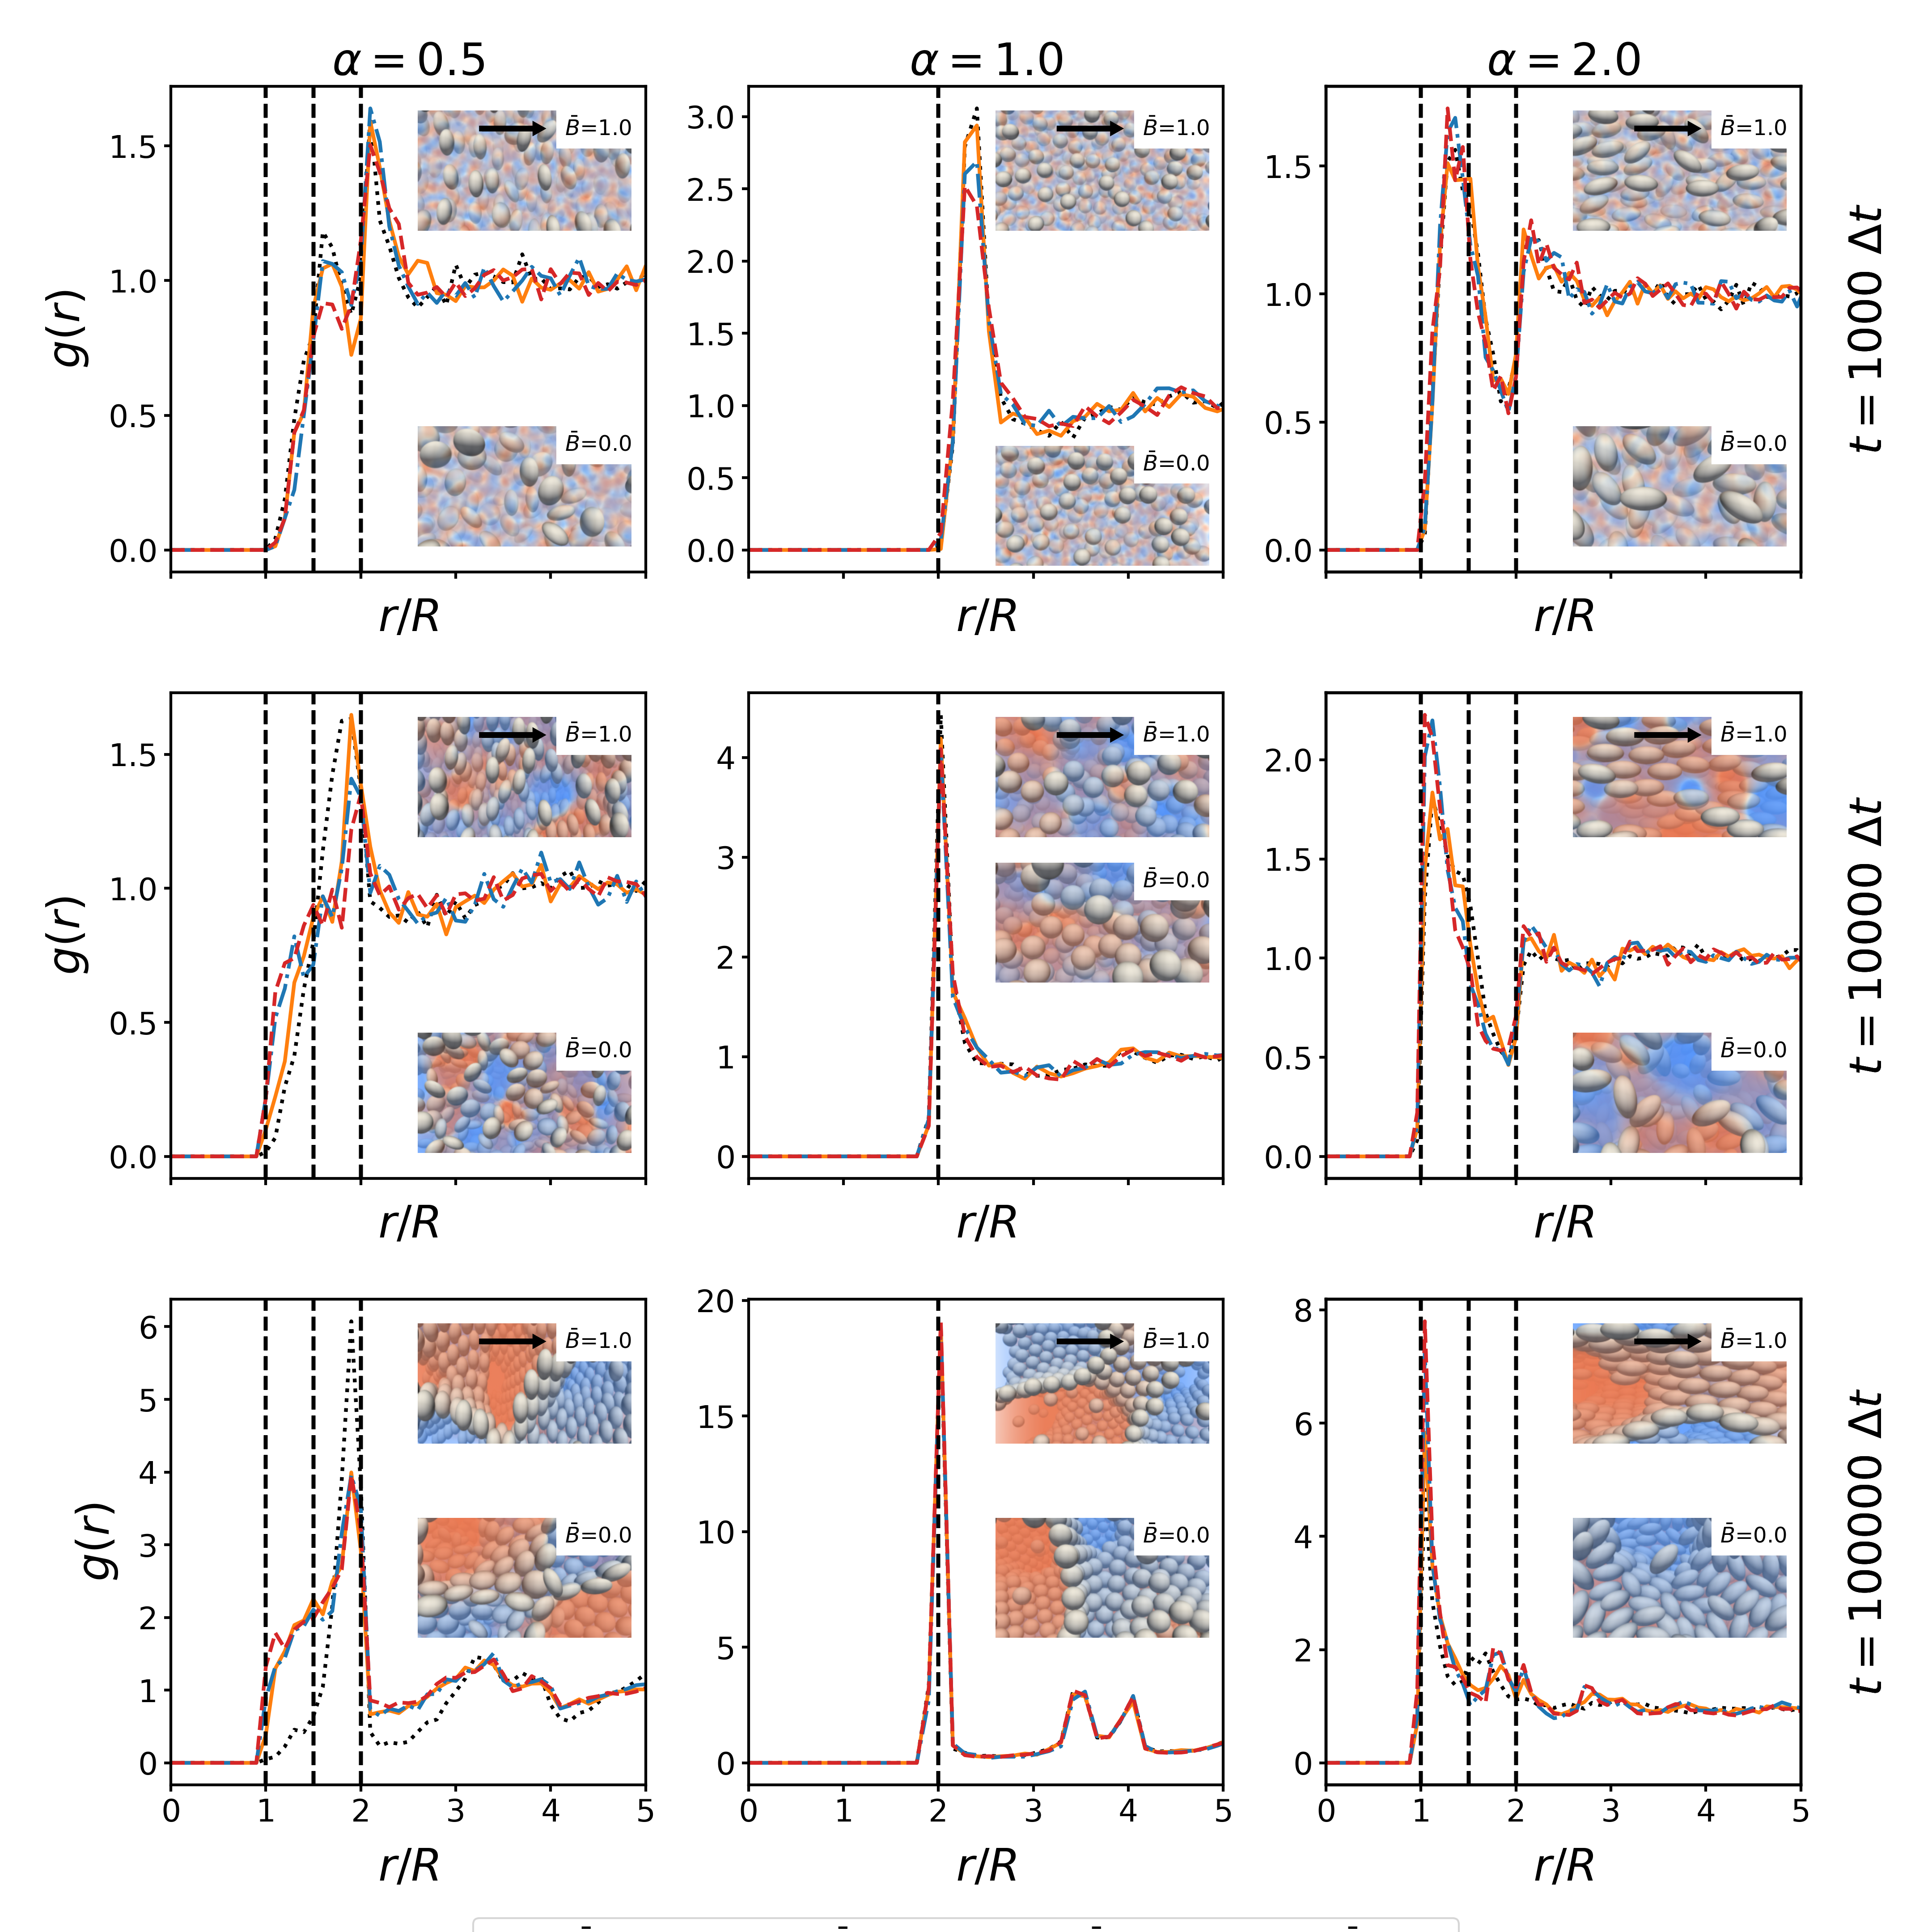
\includegraphics[width=\textwidth]{figures/results/paper1/rdf_compare_time.png}
\caption{Time-evolution of the radial distribution function $g(r)$ of the particles at different magnetic field strength $\bar{B}$. The radial distribution function is shown at $10^3$, $10^4$, and $10^5$ timesteps. The distance $r$ is normalized by the radius $R=\max(R_\parallel,R_\perp)$ of the larger particle axis. The peaks illustrate the packing of particles in the interface. Dashed lines indicate the side-by-side, tip-to-tip, and side-to-tip configuration of particle pairs. For spherical particles, the three values are identical. The insets show snapshots of the particle arrangement with and without magnetic field at the respective timesteps. The direction of the magnetic field is indicated by arrows.}
\label{fig:rdf}
\end{figure*}

The radial distribution function is shown at time steps
\(t=1000\Delta t,\ 10000\Delta t,\ 100000\Delta t\). For ellipsoidal
particles, the characteristic distances between particles in contact are
\(2R_{\parallel}\), \(2R_{\perp}\), and \(R_{\parallel} + R_{\perp}\).
These distances are marked by dashed lines in Fig. \ref{fig:rdf}. We
observe that the largest peak of the RDF coincides with the distance
\(2R_\perp\) for both oblate and spherical particles, indicating that
oblate particles tend to be in contact at their circumference while
prolate particles preferentially align side-by-side. These arrangements
lead to closer packing of particles in the interface. The peaks are less
pronounced in the early stage of the simulations, where the particles
are more randomly oriented. Notably, there is a dip in the RDF of
prolate particles at \(2R_\parallel\) indicating that initially the
tip-to-tip configuration occurs more rarely. The growth of the peak
height over time shows that the magnetic fields promote this alignment
compared to the case without magnetic field. For oblate particles, a
shoulder develops around \(R_\parallel+R_\perp\), indicating that some
particles tilt out of the interface to reduce the covered interfacial
area. For prolate particles, the dip at \(2R_\parallel\) disappears over
time, indicating that more particles align tip-to-tip. This is
consistent with alignment of prolate particles with respect to the
magnetic field, which facilitates closer packing along both axes of the
particles. It further suggests that particles arrange in layers, which can also be observed in the snapshot in Fig.
\ref{fig:packing_viz}. Together with the analysis of nematic order
above, these results substantiate the proposed mechanisms that influence
the formation of bijels with anisotropic particles in magnetic fields:
The magnetic field aligns the particle dipole axis in the field
direction, and the particle re-orientation couples to interface
alignment due to the capillary interactions. The alignment of particles
reduces the steric constraints within the interface, which allows the
interface to shrink further and facilitates domain coarsening. In terms
of the time-evolution, the rotation of particles due to the magnetic
field occurs during the initial stages of the simulation, followed by
the local re-alignment of interfaces due to capillary interactions. In
the case of prolate particles, we observed the shrinking interface can
force particles to tilt out of their preferential alignment to facilitate
closer packing. Generally, our results show that when bijels stabilized
by anisotropic magnetic particles form under the influence of a magnetic
field, the domain size and tortuosity become anisotropic. Additionally,
we observe that the particle packing in the interface becomes more
ordered due to the alignment effects.

\section{Conclusions}

In this work, we studied the effect of applied magnetic fields on the
formation of bijels stabilized by magnetic ellipsoidal particles. We
considered oblate, spherical, and prolate particles with a permanent
magnetic dipole moment suspended in a symmetric binary liquid. We found
that, while the overall formation of a bijel is not disrupted by
magnetic interactions, bijels stabilized by oblate or prolate ellipsoids
exhibit anisotropic domain size and an anisotropic tortuosity. For
oblate particles, the domain size increases in the direction
perpendicular to the magnetic field while the tortuosity increases in
the parallel direction. Conversely, for prolate particles, the domain
size increases in the direction parallel to the magnetic field while the
tortuosity increases in the perpendicular direction. Compared with
bijels formed in the absence of a magnetic field, we observed changes in
domain size up to \(30\%\) for non-spherical particles. This effect can
be explained by the re-orientation of the particle dipole axis with the
magnetic field, which in turn re-aligns the interfaces in the direction
of the longer axis of the particles. We further corroborated this
mechanisms by analyzing the coarsening speed and the nematic order of
the particles and the interfaces. We found that jamming of particles is
delayed in the direction of the longer ellipsoidal axis leading to
enhanced coarsening in this direction. The timescale of the delayed
jamming coincides with a slow-down of the orientational ordering of the
particles whereas the alignment of the interfaces increases. We also
found that the angle between the particle dipole axis and the interface
normal changes at this stage. Additionally, we analyzed the radial
distribution function of the particles and found that prolate particles
tend to align side by side, while the oblate particles exhibit a less
regular arrangement. Based on these findings, we propose that bijel
formation in magnetic fields is governed by two coupled effects: During
the initial stage, the magnetic torque rotates the particles to align
the magnetic dipole moment with the field, and the orientational order
of the particles facilitates further coarsening. As coarsening proceeds,
the capillary interactions cause the interfaces to align with the longer
particle axis. The shrinking interface compresses the particles into
ordered arrangements. When jamming sets in, some particles can be forced
to tilt out of the interface and this effect is more prominent for
oblate particles.

Our results demonstrate the effects of magnetic fields on the structural
properties of bijels stabilized by ellipsoidal magnetic particles. This
control is desirable in applications where the domain size and
tortuosity affect the transport properties. For example, reduced
tortuosity can increase the diffusive permeability of bone-like
materials \cite{prakoso2023tortuosity}. Similarly, low tortuosity
in lithium electrodes facilitates homogeneous ion transport and
uniform lithium deposition, leading to enhanced cyclability of
batteries\cite{chen_tortuosity_2020, ebner_tortuosity_2014}. Whereas we
have considered one particular regime of spinodal decomposition, the
viscosity and surface tension of the liquids offer additional parameters
that could be leveraged to tune the bijel formation. Moreover, the
particle volume fraction is another parameter that is known to affect
the formation of particle-stabilized emulsions
\cite{jansen_bijels_2011,hijnen_bijels_2015}. With respect to possible
experimental realizations of our simulations, we should emphasize that
we have generally considered micron-size particles and have neglected
thermal fluctuations. At the nanoscale, thermal fluctuations may in
principle play a role, however, Reeves et
al.~\cite{reeves_particle-size_2015} have shown that nanoparticles
benefit from smaller driving forces towards disruptive curvature and
actually lead to more robust bijel formation. Nevertheless, the
stability of magnetically-responsive bijels is a relevant question for
applications that involve shear flows such as crossflow reactors
\cite{khan_nanostructured_2022}. Aside from particle-size and shape
effects, direct interactions between particles are a possible avenue
to tune the formation of particle-stabilized emulsions gels, as the
recent discovery of bicontinuous intraphase jammed emulsion gels
(bipjels) illustrates \cite{kinkead_bicontinuous_2019}. Another
interesting observation arising from our simulations is that the
packing order of particles in the interface appears to increase when
bijels form under the influence of a magnetic field. While such
interfacial ordering effects have been studied on planar interfaces
\cite{toor_self-assembly_2016,shi_nanoparticle_2018,kim_dynamic_2022},
they have hitherto not been reported for particle-stabilized emulsion
gels. It would be interesting to examine the implications of this
ordering on the optical and transport properties of jammed emulsion
gels. In conclusion, our simulations provide relevant insights into the
formation of magnetic particle-stabilized bijels in the presence of
external magnetic fields, and they demonstrate the potential of magnetic
particles for fabrication of emulsion systems with tunable and
anisotropic particle packing and domain structure.